\chapter{Studio sull'analisi dei dati}
\label{ch:Studio sull'analisi dei dati}

\begin{citazione}
Puoi avere dati senza informazioni, ma non puoi avere informazioni senza dati. Daniel Keys Moran~\cite{daniel_keys_moran_cyte}
\end{citazione}

L'incremento dei dati, il sempre maggiore valore che stanno acquisendo e la presa di coscienza da parte delle aziende su tutti i benefici acquisibili migrando il proprio sistema in un orientamento data-driven. Questi sono solo alcune delle motivazioni che hanno portato i dati a incrementare il proprio valore e importanza all'interno del mondo. Proprio perciò con il tempo sono state diverse le tecnologie e i processi applicati a quest'ultimi per poter migliorare la loro gestione ed efficienza (e di conseguenza il valore da loro ricavabile). I più importanti tra questi sono i \textit{Big Data}, i \textit{Data Warehouse} e l'\textit{Analisi dei dati}.

\section{I Big Data}

Come accennato in precedenza le esigenze di salvataggio e gestione dei dati sono diventate sempre più importati, proprio per tale motivo ha guadagnato importanza a sua volta anche il mondo dei \textit{Big Data}. Ovvero il campo emergente in cui l’evoluzione del mondo e della sua tecnologia offre nuovi modi per recuperare il valore dalla marea di nuove informazioni generate. La capacità di gestire efficientemente le informazioni e di estrarre conoscenza da quest’ultime è diventato un vantaggio sempre più importante a cui ogni azienda aspira. Proprio per questo molte compagnie stanno basando il loro obiettivo, tanto da farlo diventare anche il proprio core business, sulla capacità di raccogliere e analizzare i dati, così da ricavare il maggior numero di informazioni utili possibili. L’adozione della tecnologia dei Big Data nell’ambito delle compagnie non può più definirsi una scelta opzionale, bensì una necessità obbligatoria per sopravvivere ed ottenere un vantaggio competitivo.\cite{new_horizon_for_a_data_driven_economy}

Questo poiché senza delle informazioni che possano considerarsi adeguate, definite tali poiché consentirebbero di svolgere scelte corrette dettate dalla conoscenza derivate dalla lettura di tali dati, difficilmente si potrebbe ottenere una strategia vincente. I Big Data sono ciò che permette di svolgere questo compito al meglio, trattandosi di beni da cui è possibile estrarre moltissime informazioni che poi potranno essere impiegate per prendere le decisioni nel miglior stato di conoscenza possibile.\cite{iusitinere_big_data}

Ad avvalorare tali affermazioni è presente il report svolto dalla piattaforma Acumen svolto a fine del 2022 (basato su dati raccolti fino al 2021), secondo cui il mercato dei Big Data a livello mondiale nel 2021 si è attestato sul valore di 165,5 miliardi di dollari. Inoltre, a seguito di approfonditi studi, è stato previsto un incremento del valore fino a 473,6 miliardi nel 2030 dovuto ad un CAGR annuale\footnote{Il \textit{Compound Annual Growth Rate} (\textit{CAGR}), o \textit{Tasso di crescita annuale composto}, corrisponde alla crescita percentuale media di una grandezza in un lasso di tempo.\cite{borsa_italiana_cagr}} del 12,7\%.\cite{acumen_big_data_market}

\begin{comment}
\begin{figure}[hbt!]
    \centering
    \includegraphics[width=1\linewidth]{figure//capitolo_3/Global-Big-Data-Market.jpg}
    \caption{Valore del mercato globale dei Big Data}
    \label{fig:Global-Big-Data-Market}
\end{figure}
\end{comment}

\subsection{Cenni storici}

Nella sua vera essenza, i Big Data non sono qualcosa di completamente nuovo o solo degli ultimi anni. Prima di approfondire l’argomento, è utile svolgere una piccola ricapitolazione su qual è stata l’evoluzione del mondo dei dati e quand’è nato il termine Big Data a cui ci riferiamo.

\begin{enumerate}
    \item La ricerca del miglioramento non è stata la sola forza a permettere al mondo di evolversi, nell’ambito della tecnologia e non, purtroppo ci sono stati anche tragici avvenimenti che hanno comportato ciò a causa della necessità di contrastarli. Ne è la dimostrazione il caso della seconda guerra mondiale, quando i tedeschi adoperarono un dispositivo chiamato Enigma per criptare i messaggi trasmessi dai loro comandi militari per evitare che potessero essere intercettati dai nemici. Gli analisti tedeschi erano convinti che per decifrare uno dei 15.576 codici sarebbe stato necessario un mese di lavoro da parte di un gruppo di matematici, tuttavia il codice di decriptazione cambiava giornalmente. Per sopperire a tale problema, il presidente degli Stati Uniti Wiston Churchill incaricò il matematico Alan Turing di gestire il centro di comunicazione cifrata per cercare di decifrare il sistema messo in piedi dai tedeschi. Per riuscire nel compito, nel 1944 Tuning propose l’utilizzo del primo computer della storia, ovvero il COLOSSUS Mk 1 inventato dall’ingegnere Tommy Flowers. Tale macchina era un calcolatore elettromeccanico capace di eseguire tutti i calcoli delle possibili combinazioni dei codici di Enigma ad altissima velocità. Fu questa una delle svolte più importanti che permise agli americani di imporsi nel conflitto.\cite{computer_history}
    \item L’importanza dei dati fu compresa fin da subito e tra i primi fautori del mondo digitale ci fu sicuramente IBM, un’azienda statunitense leader nel settore informatico, che nel 1959 creo la macchina IBM 7090, ovvero la seconda generazione del computer mainframe IBM 709 allo scopo di “applicazioni scientifiche e tecnologiche su larga scala”.\cite{wikipedia_ibm_7090}
    \item A tale evento seguì, nel 1965, la scelta del governo degli Stati Uniti d’America di eseguire l’aggregazione di dati digitali allo scopo di svolgervi un’analisi approfondita. Per svolgere tale compito decise di costruire il primo data center della storia per archiviare 742 milioni di dichiarazioni dei redditi e 175 milioni di impronte digitali. L’idea alla base era quella di trasferire le informazioni su un nastro magnetico per computer così che fossero tutte archiviate in un’unica locazione. Per quanto il compito fu poi abbandonato, questa è stata una delle azioni, perlomeno tra le prime documentate, che hanno dato inizio all’era dei dati digitali.\cite{lights_on_data_history_of_big_data}
    \item A seguito dell’idea dell’allora presidente Kennedy degli Stati Uniti d’America di permettere ad una persona di mettere piede sulla Luna, l’imprenditore Rockwell, dopo aver vinto la gara di appalto per la progettazione del razzo che permettesse agli uomini di compiere una degli eventi più importanti della storia, mostrò la necessità di un sistema automatizzato in grado di tenere traccia dell’enorme quantità di informazioni associate ai milioni di elementi che avrebbero composto la navicella in questione. Ancora una volta entrò in gioco la società IBM che nel 1968 progettò l’Information Management System (IMS), ovvero il primo database della storia. Tale sistema, ovvero un database gerarchico, fu ideato appositamente per soddisfare la richiesta fatta, riuscendoci nel migliore dei modi, diventando così importante da essere commercializzato.\cite{icm_information_management_system}
    \item Con la continuazione delle ricerche, sempre da parte di IBM, nel 1969 i ricercatori guidati da Edgar Frank “Ted” Codd rendono pubblica la loro teoria del progetto di organizzare i dati secondo un modello matematico applicato alla relazione dei dati. Da questo momento la storia dei dati verrà inevitabilmente cambiata dalla rivoluzione dei database relazionali e della loro idea della coppia entità-relazione.\cite{appunti_digitali_storia_dei_database}
    \item Nel 1989 lo scienziato informatico britannico Tim Berners-Lee propone di sfruttare la rete Internet per condividere informazioni a livello globale attraverso un sistema di "ipertesto" chiamato World Wide Web. Lo studioso avvalora con le seguenti parole la propria idea «The information contained would grow past a critical threshold, so that the usefulness [of] the scheme would in turn encourage its increased use».\cite{fp_big_data_history}
    \item Nel 1997 si è avuta la prima apparizione del termine “Big Data” nell’articolo denominato “Application-Controlled Demand Paging for Out-of-Core Visualization” scritto dai ricercatori della NASA Michael Cox e David Ellsworth. L’introduzione dell’articolo recita le seguenti parole «Visualization provides an interesting challenge for computer systems: data sets are generally quite large, taxing the capacities of main memory, local disk, and even remote disk. We call this the problem of Big Data. When data sets do not fit in main memory (in core), or when they do not fit even on local disk, the most common solution is to acquire more resources». È da questo momento che inizia ufficialmente la storia dei Big Data.\cite{researchgate_application_controlled}
    \item Nel 2000 c’è stata una prima presa di coscienza di come l’importanza dei Big Data non potesse che crescere. Ciò avvenne grazie all’economista Francis X. Diebold che presenta all’Eight World Congress of the Econometric Society un documento intitolato “I ‘Big Data Dynamic Factor Models’ per la misurazione e la previsione macroeconomica” in cui scrive le seguenti parole «Recentemente, molte ricerche scientifiche di alta qualità, che siano di natura fisica, biologica o sociale, si sono trovate a dover affrontare - e spesso ne hanno tratto vantaggio – dal fenomeno dei “Big Data”. Il termine “Big Data” si riferisce all’esplosione nella quantità (e talvolta nella qualità) dei dati disponibili e potenzialmente rilevanti, in gran parte il risultato di progressi recenti e senza precedenti nella tecnologia di registrazione e archiviazione dei dati.».\cite{citeseerx_big_data_dynamic_factor} Dimostrando in questo modo come il mondo dei dati stesse evolvendo e non potesse essere più ignorato, bensì apprezzato e sfruttato al massimo in molti ambiti.
    \item Malauguratamente, il caso della seconda guerra mondiale non è stato l’unico in cui la tecnologia è stata necessaria per risolvere problematiche di tipo bellico oppure contrastare atti di terrorismo. Ne è la dimostrazione il caso della scelta fatta nel 2004 dal comitato dell’11 settembre alle torri che, per contrastare possibili replicazioni di tali atti, unificò le numerose agenzie partecipanti accomunate dall’obbiettivo dell’antiterrorismo e le loro conoscenze in un sistema di condivisione delle informazioni basato su una rete che trascendesse i tradizionali confini governativi. Questo al solo scopo di racchiudere tutte le informazioni in un’unica fonte che permettesse di gestirli ed analizzarli nel modo più efficiente e veloce possibile.\cite{researchgate_twin_towers}
    \item Nel 2015, lo scrittore Bernard Marr cercò di mettere in luce l’importanza dei dati in un suo articolo composto per la testata giornalistica Forbes. Ai tempi con le sue parole riuscì a descrivere ciò che sarebbe avvenuto in futuro nel mondo dei dati. «I Big Data non sono una moda passeggera. Siamo appena all'inizio di una rivoluzione che toccherà ogni azienda e ogni vita su questo pianeta». Ad avvalorare la propria tesi mostrò 20 statistiche che potessero rappresentare al meglio il contesto storico del tempo. Tra tutte, una di rilevante importanza è sicuramente quella in cui affermava che solamente lo 0,5\% dei dati generati fino a quel momento fossero stati analizzati ed utilizzati, immaginando quale potesse essere il potenziale a disposizione delle persone.\cite{forbes_big_data}
\end{enumerate}

Queste, naturalmente, sono solo alcune delle testimonianze ed avvenimenti che raccontano della storia dei Big Data, riportarle tutte sarebbe pressocché impossibile data la grande importanza e vastità di tale argomento. Questi che sono solo alcuni tra i più rilevanti avvenimenti della storia ci permettono di capire come quest’ultima e l’evoluzione delle informazioni digitali si siano influenzate a vicenda. Collocando i Big Data nella loro prospettiva storica è possibile comprendere meglio come siano riusciti a raggiungere una tale popolarità e soprattutto importanza.

\begin{comment}
\begin{figure}[hbt!]
    \centering
    \includegraphics[width=0.5\linewidth]{figure//capitolo_3/Big Data Timeline.png}
    \caption{Cronologia dei Big Data}
    \label{fig:Big Data Timeline}
\end{figure}
\end{comment}

\subsection{Definizione}

Il capitolo precedente ci ha permesso di comprendere quanto sia stata rilevante l’evoluzione dei dati e di come questi abbiano inciso nella storia dell’uomo, anche al di fuori dell’ambito informatico. Facendo ciò ci è stato possibile comprendere come, anche senza un vero e proprio riferimento ad una definizione ufficiale, molti sono stati i riferimenti eterogenei al mondo dei Big Data. Per poter capire effettivamente cosa siano i Big Data bisogna quindi adoperare una definizione ufficiale, purtroppo però ad oggi non è stata ancora creata. Per questo motivo, di seguito sono riportate le più rilevanti e significative definizioni pubblicate nel tempo.

% NEW TABLE, TEST, DARIO

\begin{comment}
\begin{table}
    \centering
    \caption{Definizioni di Big Data}
    \vspace{1mm}
    
    \rowcolors{1}{graytable}{white}
    \resizebox{\linewidth}{!}{
    \begin{tabular}{c c}
        \toprule
        \rowcolor{black}
                \textbf{\textcolor{white}{Definizione}} & \textbf{\textcolor{white}{Autore}} \\
        \bottomrule
        «I Big Data sono risorse informative ad alto volume, alta velocità e/o alta varietà che richiedono nuove forme di elaborazione per consentire una migliore presa di decisioni, scoprire nuove intuizioni e ottimizzare i processi.» & Laney Doug (2001)\cite{laney_3d_data_management} \\
        «Quando le dimensioni dei dati stessi diventano parte del problema e le tecniche tradizionali per lavorare con i dati perdono efficacia.» & Mike Loukides (2010)\cite{loukides_data_science} \\
        «Dati le cui dimensioni ci costringono a guardare oltre i metodi collaudati e consolidati in quel momento.» & Jacobs Adam (2009)\cite{jacobs_big_data} \\
        «Le tecnologie Big Data rappresentano una nuova generazione di tecnologie e architetture progettate per estrarre valore in modo economico da volumi molto ampi di dati di varie tipologie, consentendo la cattura ad alta velocità, la scoperta e/o l’analisi.» & IDC (2011)\cite{idc_big_data} \\
        «I Big Data sono un insieme enorme di dati complessi che richiedono metodologie, strumenti e competenze atte a gestirli, processarli, estrarli ed analizzarli.» & Elisa Iandiorio (2021)\cite{iandorio_big_data} \\
        «Una raccolta di insiemi di dati grandi e complessi che possono essere elaborati solo con difficoltà utilizzando strumenti di gestione di database normalmente disponibili.» & Mike 2.0. (2014)\cite{mike_big_data} \\
        «Il termine “Big Data” comprende l’uso di tecniche per catturare, elaborare, analizzare e visualizzare potenzialmente grandi insiemi di dati in un periodo di tempo ragionevole non accessibile alle tecnologie informatiche standard.» & NESSI (2012)\cite{nessi_big_data} \\
        «I Big Data di solito includono insiemi di dati di dimensioni oltre la capacità dei comuni strumenti software di recuperare, pulire, gestire ed elaborare dati entro un tempo trascorso tollerabile.» & Wikipedia (2023)\cite{wikipedia_big_data} \\
        «Insiemi di dati estremamente grandi che possono essere analizzati computazionalmente per rivelare modelli, tendenze e associazioni, specialmente in relazione al comportamento umano e alle interazioni.» & Google dictionary (2023)\cite{google_big_data} \\
        «Definiamo i Big Data come un fenomeno culturale, tecnologico e accademico che si basa sull’interazione tra: (1) Tecnologia: massimizzare la potenza di calcolo e l’accuratezza algoritmica per raccogliere, analizzare, collegare e confrontare grandi insiemi di dati. (2) Analisi: trarre vantaggio da grandi insiemi di dati per identificare modelli al fine di formulare affermazioni economiche, sociali, tecniche e legali. (3) Mitologia: la diffusa convinzione che grandi insiemi di dati offrano un livello superiore di intelligenza e conoscenza che può generare intuizioni che in passato erano impossibili, con l’aura di verità, oggettività e precisione.» & danah boyd, Kate Crawford (2012)\cite{routledge_big_data} \\
        \bottomrule
    \end{tabular}
    }
    \label{tab:big_data_definitions}
\end{table}
\end{comment}

\begin{comment}
\begin{table}
    \centering
    \begin{tabular}{|p{10cm}|p{3cm}|}
        \textbf{Definizione} & \textbf{Autore} \\
        «I Big Data sono risorse informative ad alto volume, alta velocità e/o alta varietà che richiedono nuove forme di elaborazione per consentire una migliore presa di decisioni, scoprire nuove intuizioni e ottimizzare i processi.» 
        & Laney Doug (2001)\cite{laney_3d_data_management}\\
        «Quando le dimensioni dei dati stessi diventano parte del problema e le tecniche tradizionali per lavorare con i dati perdono efficacia.» 
        & Mike Loukides (2010)\cite{loukides_data_science}\\
        «Dati le cui dimensioni ci costringono a guardare oltre i metodi collaudati e consolidati in quel momento.» 
        & Jacobs Adam (2009)\cite{jacobs_big_data}\\
        «Le tecnologie Big Data rappresentano una nuova generazione di tecnologie e architetture progettate per estrarre valore in modo economico da volumi molto ampi di dati di varie tipologie, consentendo la cattura ad alta velocità, la scoperta e/o l’analisi.» 
        & IDC (2011)\cite{idc_big_data}\\
        «I Big Data sono un insieme enorme di dati complessi che richiedono metodologie, strumenti e competenze atte a gestirli, processarli, estrarli ed analizzarli.» 
        & Elisa Iandiorio (2021)\cite{iandorio_big_data}\\
        «Una raccolta di insiemi di dati grandi e complessi che possono essere elaborati solo con difficoltà utilizzando strumenti di gestione di database normalmente disponibili.» 
        & Mike 2.0. (2014)\cite{mike_big_data}\\
        «Il termine “Big Data” comprende l’uso di tecniche per catturare, elaborare, analizzare e visualizzare potenzialmente grandi insiemi di dati in un periodo di tempo ragionevole non accessibile alle tecnologie informatiche standard.» 
        & NESSI (2012)\cite{nessi_big_data}\\
        «I Big Data di solito includono insiemi di dati di dimensioni oltre la capacità dei comuni strumenti software di recuperare, pulire, gestire ed elaborare dati entro un tempo trascorso tollerabile.» 
        & Wikipedia (2023)\cite{wikipedia_big_data}\\
        «Insiemi di dati estremamente grandi che possono essere analizzati computazionalmente per rivelare modelli, tendenze e associazioni, specialmente in relazione al comportamento umano e alle interazioni.» 
        & Google dictionary (2023)\cite{google_big_data}\\
        «Definiamo i Big Data come un fenomeno culturale, tecnologico e accademico che si basa sull’interazione tra: (1) Tecnologia: massimizzare la potenza di calcolo e l’accuratezza algoritmica per raccogliere, analizzare, collegare e confrontare grandi insiemi di dati. (2) Analisi: trarre vantaggio da grandi insiemi di dati per identificare modelli al fine di formulare affermazioni economiche, sociali, tecniche e legali. (3) Mitologia: la diffusa convinzione che grandi insiemi di dati offrano un livello superiore di intelligenza e conoscenza che può generare intuizioni che in passato erano impossibili, con l’aura di verità, oggettività e precisione.» 
        & danah boyd, Kate Crawford (2012)\cite{routledge_big_data}\\
    \end{tabular}
    \caption{Definizioni di Big Data}
    \label{tab:big_data_definitions}
\end{table}
\end{comment}

\begin{comment}
\begin{figure}[hbt!]
    \centering
    \includegraphics[width=1\linewidth]{figure//capitolo_3/Big_Data.jpg}
    \caption{I Big Data}
    \label{fig:Big_Data}
\end{figure}
\end{comment}

Anche in questo caso sono state riportate le definizioni identificate come le più rilevanti, ma non tutte quelle esistenti. Ciò permette di apprendere come, per quanto non esista una definizione standard, tra tutte quelle esistenti create arbitrariamente dagli studiosi, a seguito di ampie ricerche, siano presenti delle caratteristiche comuni. Da tali tratti distintivi è possibile affermare che:

\begin{center}
\textit{Il termine Big Data fa riferimento ad un processo adoperante un insieme di dati, anche eterogenei fra loro, la cui dimensione, complessità e velocità di acquisizione ne rendono difficile la gestione, in tempi accettabili, attraverso strumenti e processi tradizionali; tuttavia, grazie ad apposite risorse (personale, hardware e software) permette di svolgere una gestione ed analisi dei dati tale da ricavare valore da questi in quantità, qualità e tempistiche prima impensabili.}
\end{center}

Quindi, è possibile semplificare il concetto dicendo che con l’espressione “Big Data” si indica la raccolta di una grande mole di dati digitali che, per acquisire valore, richiedono l’utilizzo di specifiche infrastrutture, metodologie di gestione e modelli di analisi. Come è possibile dedurre, il motivo per cui non è stato possibile creare una definizione specifica e che potesse essere assoluta è dovuto al concetto di Big Data. Poiché dipende principalmente dal fatto che si parla di una gestione ed analisi di dati che non sarebbe applicabile con tecnologie comuni, con l’evoluzione di quest’ultime dovute al passare degli anni le capacità di elaborazioni migliorerebbero e quindi non ciò che era considerato Big Data in passato potrebbe non essere considerato tale oggi o in futuro. Proprio per questo motivo la definizione di Big Data deve essere relativa e in continua evoluzione.

Sicuramente sentendo le parole “Big Data” una delle prime associazioni che si hanno nella propria mente è quella di un grande volume di dati, tuttavia se si volesse conoscere la quantità precisa per comprendere quando effettivamente si parla di Big Data ciò non sarebbe possibile per due motivi:

\begin{itemize}
    \item sono definiti “grandi” non solo per il loro volume, ma anche per la varietà e la complessità che li contraddistingue;
    \item per lo stesso motivo del “problema” che affligge la definizione del termine Big Data, non è possibile quantificare il volume minimo per parlare di Big Data poiché le dimensioni che si hanno al giorno d’oggi, come abbiamo potuto apprendere in precedenza, non sono paragonabili a quelle passate o future.
\end{itemize}

\subsection{Caratteristiche}

A seguito del proprio studio sul fenomeno dei Big Data, Doug Laney elaborò un nuovo modello in grado di definire quali fossero le loro caratteristiche. Prese il nome di “\textbf{Modello delle 3V}”, poiché pone i 3 concetti di \textit{Volume, Velocità e Varietà} alla base della definizione di Big Data (sopra riportata). Col passare degli anni e con l’evoluzione del fenomeno tale modello è stato integrato con altri quattro elementi in grado di definire e interpretare ancor di più nello specifico le caratteristiche di ogni dato, ovvero \textit{Valore, Veridicità, Valenza e Visualizzazione}. È importante precisare che risulta difficile isolare le singole caratteristiche poiché esiste una forte legame tra di loro. Di seguito sono riportate le relative definizioni.\cite{agcom_big_data}
\begin{itemize}
    \item \textbf{Volume} (\textit{Volume}). Il volume rappresenta la caratteristica che più facilmente si può accostare ai Big Data; però come detto in precedenza numerosi sono stati gli studi che cercano di misurare tale caratteristica, tuttavia è stata riscontrata l’impossibilità di conoscerne il preciso ammontare.
    \item \textbf{Varietà} (\textit{Variety}). La varietà fa riferimento all’eterogeneità delle fonti sorgenti dei dati, dei loro formati, da cui vengono acquisite le informazioni e della rappresentazione e analisi dei dati immagazzinati.
    \item \textbf{Velocità} (\textit{Velocity}). La velocità è connessa alle tempistiche con cui le banche dati vengono alimentate, in particolare alla alta frequenza con cui i dati circolano da un punto di origine a uno di raccolta. Tuttavia, la velocità non riguarda esclusivamente il flusso di dati, ma anche la necessità di processare i dati in maniera rapida e per prendere decisioni ad un ritmo sempre più veloce, spesso in tempo reale.
    \item \textbf{Valore} (\textit{Value}). Il valore corrisponde alla capacità di estrarre/ricavare dai dati il valore economico, o più precisamente le informazioni che possano diventare un valore aggiunto per svolgere decisioni, di qualsiasi genere o ambito di riferimento, che comportino un guadagno economico. 
    \item \textbf{Veridicità} (\textit{Veracity}). La veridicità pone l’attenzione sulla rilevanza degli aspetti qualitativi legati ai dati e, di conseguenza, alla fiducia che in essi si può riporre. In altri termini, la veridicità garantisce che i dati siano accurati; ciò comporta la necessità di impedire l’accumulo nei sistemi di dati che non siano “utili”.
    \item \textbf{Variabilità} (\textit{Variability}). Per prima cosa bisogna sottolineare che la variabilità è differente dalla varietà. I significati e le interpretazioni di questi agglomerati di dati grezzi dipendono molto dal loro contesto. Quando si tratta di analizzare le impressioni, questo è fondamentale. Gli algoritmi devono essere in grado di comprendere il contesto in cui operano e decifrare il significato preciso di ogni parola nel loro specifico ambiente. La variabilità illimitata dei Big Data presenta quindi una sfida di decodifica unica se si vuole sfruttare tutto il suo valore.
    \item \textbf{Visualizzazione} (\textit{Visualization}). Per visualizzazione dei dati si intende ricavare informazioni sintetiche e renderle di facile comprensione da una vastità di dati, essa rappresenta indubbiamente una delle sfide più ardue da affrontare.
\end{itemize}

\begin{comment}
\begin{figure}[hbt!]
    \centering
    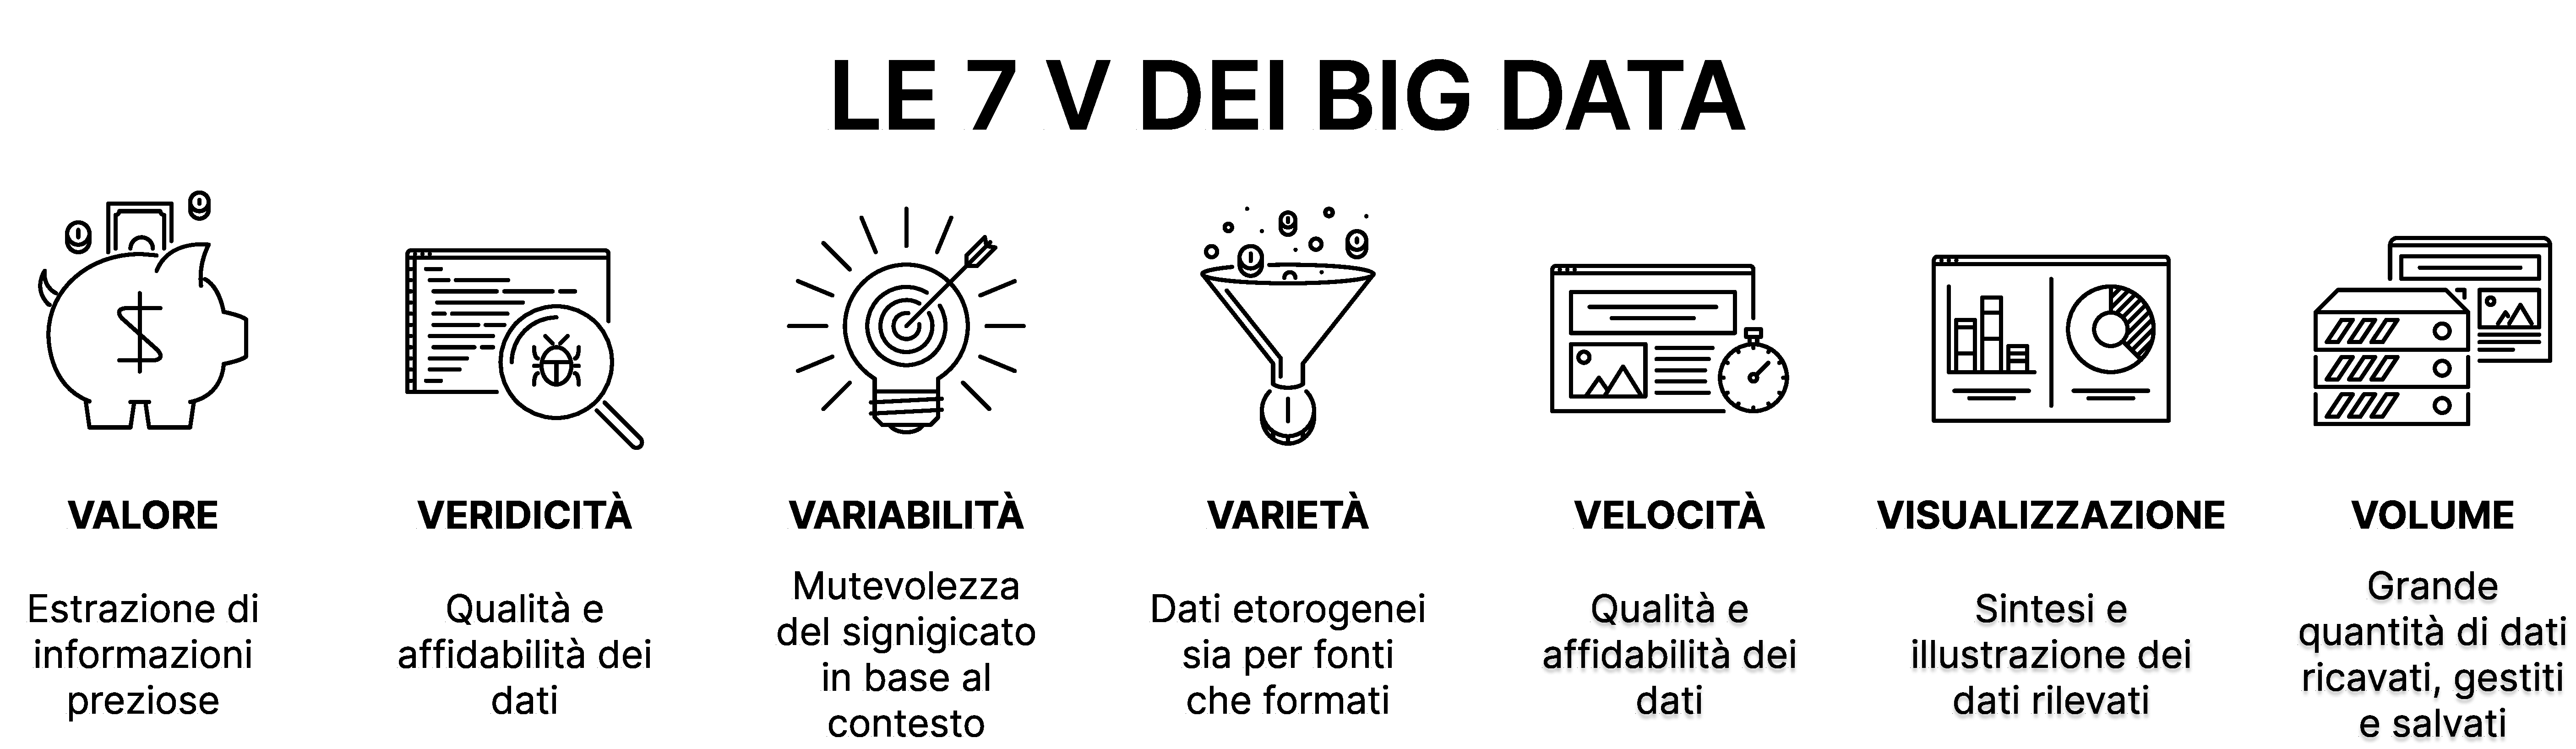
\includegraphics[width=1\linewidth]{figure//capitolo_3/Le 7 V dei Big Data.png}
    \caption{Le 7 V dei Big Data}
    \label{fig:Le 7 V dei Big Data}
\end{figure}
\end{comment}

\subsection{Strutturazione dei dati}

Come affermato sopra, una delle caratteristiche dei Big Data è la varietà poiché in un ambiente possibilmente eterogeneo come questo, i dati vengono ricevuti quasi sempre in formati differenti. In base al loro formato, o per meglio dire la loro \textit{struttura}, è necessario adoperare approcci distinti per ottenere le informazioni necessarie.

Quando si parla di \textbf{struttura dei dati} si riferisce ai metodi di organizzazione delle unità di dati all’interno di insiemi più grandi. La creazione e il mantenimento di specifiche strutture di dati aiutano a migliorare l’accesso al valore di quest’ultimi. Man mano che i dati vengono organizzati in modo più elaborato essi diventano più funzionali.\cite{theastrologypage_data_structure}

In base alle necessità, all’architettura del progetto e al loro scopo, i dati possono essere salvati in tre diversi modi:

\begin{itemize}
    \item \textbf{Dati strutturati}. I dati strutturati sono dati la cui struttura è predefinita e quindi rispettano tutti la stessa forma prima di essere inseriti all’interno dell’archivio dati. Ciò permette di avere lo stesso insieme di proprietà per i dati che rispettano il medesimo formato. Tali dati vengono anche chiamati dati relazionali poiché è possibile rappresentarli facilmente in un formato tabellare relazionabile tra loro.\cite{geeksforgeeks_big_data_structure}
    \item \textbf{Dati semi-strutturati}. I dati semi-strutturati sono una tipologia di dati che non è conforme ad una struttura formale di modelli di dati, ma che sfrutta alcuni tipi di tag organizzativi per separare gli elementi semantici che li compongono così da definire delle gerarchie per i campi che contengono le informazioni. Solitamente queste strutture sono adoperate per il salvataggio dei metadati, che contengono delle informazioni strutturate ma sempre gli stessi campi.\cite{magnimind_big_data_structure}
    \item \textbf{Dati non strutturati}. I dati non strutturati sono il tipo di dati che non aderiscono a nessuno schema o insieme di regole definito e quindi si presentano in forme o strutture sconosciute e diverse tra loro. Questo tipo di dati ha una forma sconosciuta e non può essere archiviato in modi tradizionali e non può essere analizzato a meno che non vengano trasformati in un formato strutturato. Proprio per questo motivo la gestione di tali dati è un compito impegnativo.\cite{altervista_big_data_structure}
\end{itemize}

Principalmente, i dati contenenti le informazioni vengono salvati in formati strutturati o non strutturati e per questo motivo spesso si incorre nel dubbio sul quale scegliere tra i due formati per il proprio progetto. Di seguito è riportata una tabella che mostra le differenze fra le due tipologie di dati.\cite{analytixlabs_big_data_structure}

\begin{comment}
\begin{table}
    \centering
    \begin{tabular}{ccc}
        Ambito di paragone & Dati Strutturati & Dati Non Strutturati\\
        Struttura & I dati strutturati nei Big Data si basano su RDBMS e seguono una struttura a righe-colonne. Poiché hanno sempre la stessa forma, tali dati possono essere utilizzati sia da macchine che uomini. &  I dati non sono organizzati in un modo definito, per questo motivo non funzionano con alcun set di modelli di dati. \\
        Fonti & Provengono principalmente da database relazionali, sistemi di gestione, siti web, applicazioni, dati finanziari, archivi dati, sensori e dispositivi IoT. & Provengono principalmente da file di testo, immagini, video, audio, documenti PDF, e-mail, social media, log e dati di tracciamento, documenti di elaborazione e bot di assistenza.\\
        Formati & I loro possibili formati di origini sono: CSV, Excel, Database Relazioni vari, XML, Parquet ed Avro. & I loro possibili formati di origini sono: TXT, PDF, JPEG, PNG, MP3 e MP4.\\
        Modelli & Modello che rispetta una struttura predefinita prima di essere salvati nell’archivio dati. & Sono memorizzati nel proprio formato originale senza essere elaborati finché non eseguiti.\\
        Salvataggio & I dati vengono salvati in un formato tabellare e richiedono meno spazio di archiviazione. & Questi dati vengono archiviati come file multimediali o database NoSQL, richiedendo maggiore spazio di archiviazione.\\
        Formato & Segue uno schema rigido che fornisce sia coerenza che efficienza. & Non segue una struttura costante e per questo è incoerente.\\
        Facilità di analisi & Esistono diversi strumenti di analisi rodati per il recupero, la gestione e l’analisi dei dati. & Gli strumenti per il recupero, la gestione e l’analisi dei dati sono ancora in fase di sviluppo.\\
    \end{tabular}
    \caption{Differenze tra dati strutturati e dati non strutturati}
    \label{tab:data_structure_differences}
\end{table}
\end{comment}

In altre parole, analizzando le differenze riportate nella Tabella  \ref{tab:data_structure_differences}, la scelta di adoperare uno dei due formati di dati dipende da quale sia lo scopo e soprattutto la tipologia di informazioni che si vorrebbero salvare. Non esiste un formato che prevale sull’altro in qualsiasi caso, ma solamente in base alla propria esigenza.

\begin{comment}
\begin{figure}[hbt!]
    \centering
    \includegraphics[width=1\linewidth]{figure//capitolo_3/structured-data-vs-unstructured-data.png}
    \caption{Differenze tra dati strutturati e dati non strutturati}
    \label{fig:structured-data-vs-unstructured-data}
\end{figure}
\end{comment}

\subsection{Fonti dei dati}
Naturalmente questi dati devono avere un’origine da cui essere recuperati, tali origini vengono classificate in tre differenti macro-categorie:\cite{upgrad_big_data_sources}

\begin{itemize}
    \item \textit{Machine data}.Sono dati auto generati a seguito di un evento registrato da parte di un sistema oppure di una pianificazione precedentemente determinata. Principalmente questi dati derivano da dispositivi IoT, sensori smart, dispositivi medici o indossabili, satelliti, dispositivi tecnologici di vario genere. Tali fonti permettono di monitorare il comportamento degli utenti che si interfacciano ad essi. I dati così generati crescono in modo esponenziale sia grazie all’aumento di interazioni che di dispositivi fruibili. Inoltre, in un contesto più ampio, è possibile includere in questa categoria anche i dati derivanti da server, applicazioni utente, siti web, programmi SaaS, eccetera.
    \item \textit{Social data}. Come è possibile intuire, questi sono i dati che vengono generati da tutti i social media a disposizione degli utenti come ad esempio commenti, mi piace, messaggio, foto, video, ecc. insomma qualsiasi tipo di interazione svolta su tali piattaforme. Una volta sviluppati, tali dati offrono importanti approfondimenti qualitativi e quantitativi per le aziende su ogni aspetto riguardante il collegamento con il proprio pubblico. Essendo le piattaforme social degli ambienti dove lo sviluppo delle interazioni e quindi di ulteriori informazioni aumenta vertiginosamente ogni giorno, le aziende cercano di sfruttarle al meglio per scopi commerciali che permettano di migliorando la propria conoscenza delle preferenze dell’utenza a cui fanno riferimento.
    \item \textit{Transactional data}. Essi sono i dati riguardanti le informazioni raccolte tramite transazioni, sia online che offline, svolte da varie applicazioni per l’esecuzione di processi aziendali atti all’acquisto o alla vendita di un prodotto. Tali dati includono informazioni importantissime come l’ora della transazione, la posizione, il prodotto acquistato, il relativo prezzo, il metodo di pagamento e molto altro, insomma ogni genere di informazione sensibile di ambito economico. Questi non solo sono le informazioni di maggior valore, ma inoltre delle varie categorie probabilmente sono quelli con il più alto incremento ed evoluzione al mondo, data la loro grande importanza.
\end{itemize}

\subsection{Catena del valore (Data Value Chain)}
Generare del valore è l’obbiettivo alla base di qualsiasi organizzazione. Tuttavia, in un mondo che cambia, in termini di dati, è molto difficile trovare strategie per generare nuovo valore in modo sostenibile e migliorare le operazioni. Per questo motivo, ogni azienda deve garantire una gestione efficiente e sempre aggiornata dei processi di generazione del valore sia per l’organizzazione stessa che per i propri partner. La \textbf{catena del valore} \textit{(Value Chain, VC}) è una delle soluzioni chiave a tale dilemma.\cite{springer_big_data_value_chain}
Ideata da Michael Porter\cite{porter_big_data_value_chain}
, la catena di valore consiste nell’analizzare tutte le attività e le loro relative interazioni, identificare le fonti di un potenziale vantaggio competitivo e organizzare i processi che contribuiscono direttamente o indirettamente alla creazione di valore aggiunto per la compagnia.\cite{wiley_big_data_value_chain}

La VC era uno strumento indispensabile per permettere l’analisi delle interazioni tra attività differenti per identificare dove il valore ricercato potesse essere generato. Tuttavia, con l’avvento della digitalizzazione, è stato necessario evolvere anche il modello della value chain ormai obsoleto, mettendo le informazioni dei dati digitali alla base del proprio principio, prendendo così il nome di \textit{Data Value Chain} (\textit{DVC}).\cite{core_data_value_chain} Proprio grazie a questo motivo, il modello della catena di valore ha guadagnato sempre più importanza.

Come descritto da Edward Curry, la Data Value Chain si compone delle cinque seguenti attività\cite{curry_data_value_chain}:

\begin{enumerate}
    \item \textbf{Acquizione dei dati} (\textit{Data Acquisition}). Corrisponde al processo di raccolta, filtraggio e pulizia dei dati prima che vengano inseriti all’interno del sistema di archiviazione designato. L’acquisizione dei dati è una delle sfide più importanti legate all’ambito dei Big Data e dei suoi requisiti infrastrutturali. Il sistema preposto per il mantenimento dei dati deve garantire una latenza bassa e prevedibile, sia in caso di scrittura che lettura, per grandi volumi di dati.
    \item \textbf{Analisi dei dati} (\textit{Data Analysis}). Tale attività si occupa di trasformare i dati grezzi acquisiti in formati utilizzabili durante il processo decisionale oppure utilizzabili per uno specifico ambito. L’analisi dei dati implica l’esplorazione, la trasformazione e la modellazione dei dati con l’obiettivo di evidenziare dati rilevanti, così da estrarre e sintetizzare le informazioni utili presenti nei dati.
    \item \textbf{Cura dei dati} (\textit{Data Curation}). Per cura dei dati si intende la gestione attiva dei dati durante il loro ciclo di vita, garantendo così che quest’ultimi soddisfino i requisiti di qualità dei dati necessari per un loro efficace utilizzo.  I processi di data curation possono essere classificati in diverse attività come la creazione, la selezione, la classificazione, la trasformazione, la convalida e la conservazione dei contenuti. Proprio per questo motivo tale attività viene eseguita da personale esperto.
    \item \textbf{Salvataggio dei dati} (\textit{Data Storage}). Il processo di data storage riguarda la persistenza e la gestione dei dati in modo scalabile che soddisfa le esigenze delle applicazioni che richiedono un accesso rapido ai dati. In questo ambito, i \textit{sistemi di gestione dei database relazionali} (\textit{Relational Database Management System, RDBMS}) rappresentino la soluzione principale, e quasi unica. Tuttavia, le proprietà \textit{ACID} (\textit{Atomicity, Consistency, Isolation and Durability}, ovvero \textit{Atomicità, Consistenza, Isolamento e Durabilità}) che garantiscono le transazioni dei database mancano di flessibilità per quanto riguarda le modifiche dello schema e le prestazioni e la tolleranza agli errori quando i volumi e le complessità dei dati crescono, rendendole inadatte per scenari dei Big Data.
    \item \textbf{Uso dei dati} (\textit{Data Usage}). L’ultima attività, ovvero l’uso dei dati, rappresenta le attività aziendali basate sui dati che richiedono l’accesso ai dati, la loro analisi e gli strumenti necessari per integrare l’analisi dei dati all’interno dei processi decisionali. Ciò permette di migliorare la competitività attraverso la riduzione di costi, l’aumento del valore aggiunto o qualsiasi altro parametro che possa essere misurato rispetto ai criteri di prestazione preesistenti.
\end{enumerate}

\begin{comment}
\begin{figure}[hbt!]
    \centering
    \includegraphics[width=0.75\linewidth]{figure//capitolo_3/Big Data Value Chain.png}
    \caption{Big Data Value Chain}
    \label{fig:Big Data Value Chain}
\end{figure}
\end{comment}

\subsection{Vantaggi e problematiche dei Big Data}

I Big Data rappresentano il fattore produttivo chiave in un’economia data-driven; molti sono gli ambiti, sia provati che pubblici, in cui l’utilizzo di tecniche di analisi di big data ha permesso di creare nuovi servizi, migliorare quelli esistenti, innovare i processi produttivi e distributivi, rendere l’offerta di tutti i prodotti e servizi, migliorare quelli esistenti, innovare i processi produttivi e distributivi, rendere l’offerta di tutti i prodotti e servizi (anche non digitali) più rispondenti alle esigenze dei consumatori e cittadini. Tuttavia, benché stimolante, l’analisi dei big data è un’operazione complessa. I data scientist si occupano dell’analisi dei dati per offrire all’azienda informazioni e raccomandazioni utili e i data engineer sono responsabili di identificare, assemblare e gestire gli strumenti necessari in un flusso di dati. Ogni singola fase rappresenta delle sfide in termini di integrazione, capacità di storage e riduzione dei budget IT.\cite{redhat_big_data}

Pertanto di seguito sono riportate alcune delle problematiche che bisognerebbe considerare se si ha l’intenzione di predisporre un sistema per l’applicazione dei Big Data\cite{microsoft_big_data}:

\begin{itemize}
    \item \textit{Organizzazione e accessibilità dei dati}. La principale problematica associata ai Big Data consiste nel capire come gestire il volume di informazioni ottenute affinché pervengano correttamente nelle applicazioni.
    \item \textit{Controllo qualità}. Garantire l’accuratezza e la qualità dei dati può essere difficile e dispendioso in termini di tempo, soprattutto quando tali dati arrivano rapidamente e a volumi molto elevati. Prima di effettuare qualsiasi analisi, occorre assicurarsi che i processi di raccolta, elaborazione e pulizia dei dati siano integrati, standardizzati e ottimizzati.
    \item \textit{Sicurezza dei dati}. Con l’aumento delle violazioni di dati, la protezione di quest’ultimi ha sempre più importanza. Così come il sistema di analisi cresce, aumenta anche la possibilità di riscontrare problemi di sicurezza sotto forma di dati fittizi, fughe di informazioni, problematiche relative alla conformità e alla vulnerabilità del software. Per ridurre alcune di tali preoccupazioni, occorre crittografare i dati e condurre regolarmente controlli di sicurezza.
    \item \textit{Scelta degli strumenti giusti}. Dover scegliere tra i tantissimi strumenti e tecnologie disponibili può creare confusione. Ecco perché è importante provvedere alla formazione, rimanere sempre aggiornati e, se possibile, assumere o consultare uno specialista ove necessario.
\end{itemize}

Una volta mostrare le problematiche a cui fare attenzione per sviluppare un sistema di gestione dei Big Data, è ora importante mostrare quanto siano rilevanti i vantaggi nell’intraprendere questa scelta.\cite{oracle_big_data}

\begin{itemize}
    \item \textit{Sviluppo di prodotti e servizi}. L’analisi dei Big Data consente agli sviluppatori di prodotti di analizzare dati non strutturati, quali le recensioni dei clienti e le tendenze culturali, e di reagire prontamente anche predicendo le eventuali richieste anticipando la domanda della propria utenza.
    \item \textit{Manutenzione predittiva}. I fattori che possono prevedere guasti meccanici possono essere nascosti tra i dati strutturati, riguardanti le informazioni della strumentazione, oppure nei dati non strutturati, riguardanti le informazioni generate da tali dispositivi. Analizzando queste indicazioni di potenziali problemi prima che si verifichino, le aziende possono svolgere la manutenzione in modo più efficiente in termini di costi e tempistiche.
    \item \textit{Customer Experience}. I Big Data consentono di raccogliere dati da social media, visite sui siti web, registri delle chiamate e altre fonti allo scopo di migliorare l’esperienza di interazione tra l’utente e l’azienda. In altre parole, l’analisi di tali dati permette alle organizzazioni di migliorare l’esperienza vissuta dai clienti con il loro brand in modo da ottenere una maggiore soddisfazione da parte dell’utente, che corrisponde a possibili nuovi introiti.
    \item \textit{Frode e conformità}. Gli scenari di sicurezza e i requisiti di conformità sono in continua evoluzione. I Big Data aiutano a identificare i modelli nei dati che indicano frodi e ad aggregare grandi volumi di informazioni per rendere i rapporti normativi molto più veloci. Gli insight generati dall’analisi dei tali dati consentono alle aziende di anticipare il rischio e a prepararsi ad eventuali malevoli imprevisti.
    \item \textit{Efficienza operativa}. L’efficienza operativa potrebbe non essere sempre un argomento innovativo, ma ha molta rilevanza nel mondo dei Big Data. In tale ambito, è possibile analizzare e valutare la produzione, i feedback e i resi da parte dei clienti, e ulteriori fattori per ridurre le interruzioni e anticipare le future richieste. I big data possono essere utilizzati anche per migliorare il processo decisionale in linea con l’attuale domanda di mercato.
    \item \textit{Incentivare l’innovazione}. I Big Data possono aiutare ad innovare studiando le interdipendenze tra essere umani, istituzioni, entità e processi e quindi determinando nuovi modi per utilizzare tali insight. Sfruttare gli insight così generati crea infinite possibilità, dal migliorare le decisioni su considerazioni interne a fornire nuovi prodotti e servizi.
\end{itemize}

\subsection{Tipologie di strumenti disponibili sul mercato}
Come affermato in precedenza dotarsi di strumenti avanzati è tanto importante quanto difficile, poiché per molte aziende potrebbe essere complicato individuare la migliore tecnologia di gestione ed analisi dei Big Data. Per questo motivo è utile potersi fare un’idea, almeno, della loro categorizzazione così da comprendere meglio quale possa essere la scelta più congeniale per le proprie esigenze. In linea generale gli strumenti disponibili sul mercato possono essere suddivisi in tre categorie principali:\cite{sadas_big_data}

\begin{itemize}
    \item \textit{Aggregatori}. Sono gli strumenti che si occupano di raccogliere e organizzare i dati provenienti da fonti eterogenee, sia interni che esterni all’azienda. Tali dati vengono poi strutturati, integrati e ordinati in modo da poter essere poi utilizzati a supporto dei processi decisionali. Queste soluzioni sono utili e necessarie per le compagnie che fanno parte di multipli mercati e quindi hanno l’esigenza di gestire varie tipologie di dati.
    \item \textit{Arricchitori}. Sono gli strumenti che pre-elaborano i dati al fine di estrapolare informazioni specifiche in linea con le necessità aziendali. Tale pre-elaborazione consiste nel recuperare delle informazioni mirate a determinati bisogni a cui vengono associate ulteriori informazioni derivanti da fonti esterne per poterli arricchire ulteriormente. Questi strumenti vengono adoperati per segmentare il mercato, profilare la clientela così da poter personalizzare il più possibile le strategie aziendali e rivolgersi ad un target più consono al proprio ambito di applicazione.
    \item \textit{Modellatori}. Sono gli strumenti che hanno come finalità quella di creare modelli di previsione tramite l’utilizzo di algoritmi che evidenziano schemi e correlazioni tra i dati. Questa categoria può essere utile per comprendere meglio i propri clienti, prodotti e partner così da identificare i rischi e le opportunità per un’azienda.
\end{itemize}

\subsection{Ambiti di applicazione}
Come espresso più volte nei paragrafi precedenti, gli ambiti di applicazioni dei Big Data sono molto ampi, di seguito eccone riportati alcuni:\cite{sciencedirect_big_data_technologies}

\begin{itemize}
    \item \textit{Smart Grid}. Gestire in tempo reale il consumo elettrico nazionale e monitorare il funzionamento delle \textit{smart grid}\footnote{Una \textit{smart grid} (o \textit{rete intelligente}, è un sistema di rete elettriche che adopera tecnologie digitali e altre tecnologie avanzate per monitorare e gestire il trasporto dell’elettricità da tutte le fonti di generazione per soddisfare le diverse richieste di elettricità degli utenti finali.\cite{iea_smart_grid}} è un compito fondamentale. Ciò si ottiene attraverso molteplici connessioni tra dispositivi, sistemi e sensori smart associati a centri di controllo e altre apposite infrastrutture. L’analisi dei Big Data aiuta a identificare possibili compenti a rischio di malfunzionamento e a rilevare dei comportamenti anomali dei dispositivi collegati. L’analisi in tempo reale dei Big Data generati consente di modellare scenari di incidenti, consentendo di stabilire eventuali piani preventivi.
    \item \textit{E-Health}. I settori della medicina e della salute sono sempre più una parte integrante della digital trasformation e in futuro potrebbero svilupparsi ulteriormente; l’evoluzione di tale mondo, ha preso il nome di E-Heath\footnote{Con il termine "\textit{E-Health}" si intende il modello di organizzazione del sistema sanitario basato sull’integrazione di strumenti e risorse telematiche e i dati relativi a ciascun cittadino\cite{treccani_ehealth}}. L’analisi avanzata dei set di dati medici ha molte applicazioni vantaggiose. Consente di personalizzare i servizi sanitari, adattare i piani sanitari pubblici in base ai sintomi della popolazione, all’evoluzione della malattia e ad altri parametri. Inoltre, è molto utile per ottimizzare le operazioni ospedaliere e ridurre la spesa sanitaria.
    \item \textit{Internet of Things}. Questo è sicuramente uno dei principali mercati dell’applicazione dei Big Data. A causa dell’elevata varietà di dispositivi, le applicazioni dell’IoT\footnote{Il termine \textit{IoT}, o \textit{Internet of Things}, fa riferimento alla rete collettiva di dispositivi connessi e tecnologie che facilita la comunicazione tra dispositivi e cloud, nonché tra i dispositivi stessi.\cite{aws_iot}} sono in continua evoluzione e generano sempre più dati grezzi. Fornendo sistemi di filtraggio, ordinamento ed analisi dei dati, il mondo dei Big Data ben si sposa con quello dell’IoT che necessità di una sempre maggiore gestione dei dati generati. Proprio allo scopo di evolvere sempre di più, l’unione di questi due mondi è alla base delle idee di sviluppo per l’industria pensando ad esempio a casi di applicazione come le smart city.
    \item \textit{Servizi Pubblici}. Un perfetto esempio dell’applicazione dei Big Data nell’ambiente dei servizi pubblici, quanto mai contemporaneo, riguarda le organizzazioni di approvvigionamento idrico che adoperano sensori nelle condutture per monitorare il flusso dell’acqua onde evitare sprechi in un periodo di carenza. Inoltre, sempre parlando dell’ambito delle aziende per la gestione degli impianti idrici, grazie ad un’analisi in tempo reale dei sensori è possibile identificare e riparare tempestivamente i tubi dell’acqua che subiscono rotture, perdite o simili.  
    \item \textit{Trasporti e logistica}. Molte aziende di trasporto pubblico su strada utilizzano l’RFID (Radiofrequency Identification, identificazione a radiofrequenze) e il GPS per tracciare gli autobus e rilevare dati interessanti per migliorare i servizi elargiti. Inoltre, sono stati implementati vari sistemi in tempo reale non solo per fornire consigli ai passeggeri ma anche per offrire preziose informazioni su quando aspettare il prossimo autobus per una determinata destinazione. Senza contare che l’estrazione dei Big Data aiuta anche a migliorare il business dei viaggi prevedendo la domanda di reti pubbliche o private.
    \item \textit{Servizi Politici e monitoraggio del governo}. Molti governi, come l’India e gli Stati Uniti, stanno estraendo dati per monitorare le tendenze politiche e analizzare i sentimenti della popolazione. Esistono molte fonti da cui recuperare tali dati: interazioni sui social network, interviste personali e le composizioni degli elettori. Tali sistemi consentono anche di individuare problematiche locali oltre a quelle nazionali e di ottimizzare l’uso di risorse e servizi preziosi.
\end{itemize}

\subsection{Small data}

Per quanto finora sono stati l’argomento portante è importante sottolineare che non esistono unicamente i Big Data, anzi, a quest’ultimi si contrappongono gli small data dopo una serie di interrogativi atti a comprendere la validità dei primi e quanto potessero essere corrette le analisi prodotte su una mole di dati indifferenziati. Gli small data permettono di ottenere informazioni più precise, rivelandosi molto affini all’ambito dell’aderenza e della verosimiglianza ai modelli reali; come è intuibile, sono dati di piccole dimensioni ma ben strutturati. Ovviamente, con il loro utilizzo, il nodo cruciale risiede nell’eseguire in maniera corretta l’analisi e non nella capacità, permettendo in questo modo di diminuire i rischi che possono esserci nell’analisi di una grande mole di dati.\cite{selcoerp_small_data}

A livello pratico il concetto di small data fa riferimento a tutta una serie di dati individuali e unici relativi a singole persone, nello specifico ad abitudini e azioni più o meno consapevoli che le persone compiono nella loro vita quotidiana. Se osservati e analizzati, tutti questi comportamenti particolari possono costituire in ottica aziendale informazioni rilevanti sulle emozioni, sui bisogni e sugli interessi dei potenziali consumatori consentendo di integrarle con strategie di marketing emozionale\footnote{Il termine "\textit{marketing emozionale}" si riferisce agli sforzi pubblicitari che fanno leva sulle emozioni per fare in modo che le persone notino, ricordino, condividano e comprino un determinato prodotto o servizio.\cite{oberlo_marketing_emozionale}}.\cite{italiaonline_small_data}

\subsubsection{Le sette fasi degli Small Data}

Il principale teorico degli Small data, ovvero Martin Lindstrom, ha definito nel proprio libro\cite{lindstrom_small_data} un modello in sette passaggi, denominato le 7C, per la raccolta e l’analisi di questi particolari dati. Alla base di questo modello si pone l’idea per cui esisterebbero tra le 500 e le 1000 tipologie di persone diverse, influenzate da quattro fattori differenti: il clima, il governo, la religione e le tradizioni. Di seguito sono riportati i sette passaggi:
\begin{enumerate}
    \item \textit{Collecting} (\textit{Raccolta}). In questa fase si ha l’obiettivo di raccogliere la maggior quantità di dati possibile, proveniente da diverse prospettive, così da astrarre l’informazione rispetto al contesto di vita da cui deriva tale nozione.
    \item \textit{Clues} (\textit{Indizi}). In questa fase si ha l’obiettivo di raccogliere indizi, facendo domande, cercando di rilevare gli elementi riguardanti la vita privata delle persone. Ciò avviene grazie alla comprensione delle loro reazioni emotive rispetto alla creazione di una narrazione su ciò che sta avvenendo.
    \item \textit{Connecting} (\textit{Connessione}). In questa fase si ha l’obiettivo di sfruttare quanto ricavato nelle fasi precedenti per ricavare i punti in comune o qualcosa che definisca una direzione ben precisa.
    \item \textit{Causation} (\textit{Ricerca} di una causa). In questa fase si ha l’obiettivo di svolgere un’analisi per comprendere le relazioni causa-effetto indagando sulle emozioni delle persone.
    \item \textit{Correlation} (\textit{Correlazione}). In questa fase si ha l’obiettivo di comprendere quale sia stato il momento in cui tale emozione/comportamento è emerso per la prima volta nella persona in analisi.
    \item \textit{Compensation} (\textit{Compensazione}). In questa fase si ha l’obiettivo di ricercare quale sia il desiderio inappagato che è alla base del comportamento della persona in questione e quale sia il miglior modo per soddisfarlo.
    \item \textit{Concept} (\textit{Concetto}). In questa fase si ha l’obiettivo di mettere in chiaro l’idea da parte dell’azienda che permetta di appagare il desiderio della persona, e quindi dell’eventuale cliente.
\end{enumerate}

Come è possibile comprendere, l’approccio ideato da Lindstrom è un processo che aiuta a comprendere meglio i consumatori, identificare i loro desideri inappagati e generare delle idee che si basino su questi per migliorare le strategie di marketing rendendole più efficaci e mirate.

\begin{comment}
\begin{figure}[hbt!]
    \centering
    \includegraphics[width=0.5\linewidth]{figure//capitolo_3/The 7C of Small Data.png}
    \caption{Le 7C degli Small Data}
    \label{fig:The 7C of Small Data}
\end{figure}
\end{comment}

\subsection{Thick data}

Come abbiamo potuto comprendere dal precedente sotto capitolo, i Big Data non riescono a mostrare tutte le informazioni che si potrebbero recuperare da una determinata fonte. Nel caso degli small data è possibile recuperare la “parte emotiva”, corrispondente a sue volta in ulteriori informazioni adoperabile per diventare conoscenza ed essere infine sfruttate. Allo stesso modo, esiste un’altra famiglia di dati che ha la sua rilevanza nel mondo dell’analisi dei dati, ovvero i thick data.

I thick data riguardano le informazioni sul significato e le connessioni che le persone attribuiscono ai servizi o alle tecnologie, così come il processo con cui li consumano. L’idea alla base è che l’analisi interpretativa dei dati deve seguire un approccio non solamente quantitativo ma anche qualitativo puntando a ulteriori fattori come quelli esterni ai dati a disposizione. Di seguito è riportata una tabella riepilogativa che permette di comprendere la differenza tra i Big Data ed i Thick Data.\cite{big_data_and_thick_data}
\begin{comment}
\begin{table}[!ht]
    \centering
    \caption{Differenza tra i Big Data e i Thick Data}
    \begin{tabular}{|l|l|l|}
    \hline|
        \textbf{Caratteristiche} & \textbf{Big Data} & \textbf{Thick Data} \\ \hline
        Formato & Dati in formato numerico. & Dati non numerici, qualitativi formato. \\ \hline
        Volume & Solitamente quantità elevate. & Solitamente quantità basse. \\ \hline
        Metodi di collezione & Documenti digitali, archivio digitalizzato record, streaming di dati, log di trasmissione, dati numerici recuperati da Internet. & Osservazioni e interviste dirette ai partecipanti, focus group, sondaggi a risposta aperta, video registrazioni, dati qualitativi provenienti da Internet \\ \hline
        Analisi & Ricerche di scienziati sociali e computazionali. & Ricerche di antropologi e etnografi. \\ \hline
        Requisito di immersione & Non è necessario che gli analisti siano in loco per analizzare i dati. & Di solito in loco o con l'osservazione diretta online, e immersi nel contesto. \\ \hline
        Ruolo nella soluzione dei problemi & Generare soluzioni a problemi in gran parte noti, generando decisioni automatiche. & Identifica i problemi che contano di più per le parti interessate e testa le soluzioni prima di espanderle. \\ \hline
        Punti di forza & \textit{Scala}: generare insight generalizzabili a un’ampia porzione o a un’intera popolazione. & \textit{Profondità}: identificare ciò che interessa in primo luogo agli stakeholder; dipingere un quadro olistico di determinate esperienze. \\ \hline
    \end{tabular}
    \label{BG vs TD}
\end{table}
\end{comment}

In altre parole, i thick data permettono di comprendere le motivazioni che hanno portato le persone a svolgere determinate scelte, ciò permette anche di comprendere quali sono stati i ragionamenti e le sensazioni che hanno portato a prendere una determinata decisione da parte di un utente. Di conseguenza, quando i Big Data vengono combinati con i thick data, è possibile generare un quadro più completo delle esigenze, dei requisiti e delle preferenze dei consumatori.

\begin{comment}
\begin{figure}[hbt!]
    \centering
    \includegraphics[width=0.75\linewidth]{figure//capitolo_3/Thick and Big Data.jpeg}
    \caption{Schema dei Thick e Big Data}
    \label{fig:Thick and Big Data}
\end{figure}
\end{comment}

\subsection{Differenza tra i Big Data e i dati tradizionali}

Di seguito è riportata una tabella che permette di descrivere le differenze tra i Big Data e i dati tradizionali.\cite{big_vs_traditional_data}

\begin{comment}
\begin{table}
    \centering
    \begin{tabular}{ccc}
        Caratteristica & Big Data & Dati tradizionali\\
        Dimensioni & Volumi approssimativamente misurati in petabyte, exabyte o zettabyte. & Volumi approssimativamente misurati in gigabyte e terabyte\\
        Organizzazione & Dati, principalmente, grezzi o non strutturati con schemi dinamici & Dati strutturati organizzati in record, file e tabelle, solitamente sono dati relazionali\\
        Architettura & Quasi sempre gestiti adoperando sistemi distribuiti dato il volume e la complessità & Solitamente gestiti adoperando sistemi con strutture centralizzate\\
        Fonti & Derivano da fonti di qualsiasi genere: programmi, social media, dispositivi IoT, ecc. & Derivano in genere da determinati programmi con uno scopo specifico\\
        Analisi & L’analisi può essere svolta sia in modo incrementale che in tempo reale & Analisi incrementale: si verifica un evento, i dati vengono generati, gestiti e poi analizzati\\
    \end{tabular}
    \caption{Differenza tra Big Data e dati tradizionali}
    \label{tab:big_vs_traditional_data}
\end{table}
\end{comment}
I Big Data e i dati tradizionali hanno scopi diversi ma correlati, che ben possono collaborare tra loro.

\section{I Data Warehouse}

Il \textit{data warehousing} ha iniziato il proprio percorso negli anni ’70 grazie a William H. Inmon e Ralph Kimball poiché ritenevano che i database basati sui modelli, per quanto efficienti nel trattamento dei dati relazionali, non lo erano altrettanto per casi di report analitici complessi. Le aziende necessitavano di una maggiore analisi dei dati per prendere decisioni aziendali efficaci e ben ragionate. Ai tempi non esisteva una metodologia di integrazione adeguata disponibile per rappresentare i dati necessari che le compagnie immagazzinavano nei vari sistemi di supporto.\cite{researchgate_data_warehouse}
Per sopperire a tali necessità Inmon e Kimball condussero una ricerca dettagliata sui sistemi di supporto decisionale e sui data warehouse, sviluppando un loro approccio nella creazione di tali sistemi che permettessero attività di analisi, centralizzando grandi quantità di dati derivanti da più origini e formati.

\subsection{Definizione}

Il padre del termine \textbf{data warehouse} è William H. Inmon che, nel finire degli anni ’90, lo definisce come «una raccolta di dati orientati al soggetto, integrati, non volatili e varianti nel tempo, finalizzata a supportare le decisioni della direzione aziendale». In quest’ottica, i data warehouse assumono un doppio scopo nella gestione dei dati:\cite{inmon_building_the_data_warehouse}

\begin{itemize}
    \item Possibilità di essere interrogati per recuperare specifiche informazioni necessarie nell’immediato.
    \item Mantenimento dei dati con l’obiettivo di sfruttarli in futuro quando avranno assunto maggior valore.
\end{itemize}

\subsubsection{Le caratteristiche}

Facendo riferimento alla suddetta definizione di Inmon, è possibile affermare che essa si basi su quattro caratteristiche fondamentali che riguardano i dati di cui un data warehouse si compone, per avere una migliore comprensione del concetto di seguito sono riportate le spiegazioni di tali caratteristiche:\cite{researchgate_data_warehouse_architecture}

\begin{enumerate}
    \item \textit{Orientati al soggetto}: tutti i dati, ritenuti importanti, relativi ad un determinato argomento vengono raccolti e archiviati come un unico insieme in un formato utile; tali dati vengono presentati in base a soggetti specifici oppure aree di interesse.
    \item \textit{Integrati}: i dati vengono archiviati in modo globalmente accettabile, ovvero rispettando una determinata convenzione cosicché le loro strutture e attributi possano essere coerenti anche indipendentemente dal caso in cui il loro formato originale di archiviazione, dovuto a sistemi operativi eterogenei, siano differenti o addirittura incompatibili.
    \item \textit{Non volatili}: le informazioni ricavabili dai dati archiviati non devono cambiare ogni volta che viene eseguito un processo di recupero o analisi; tali informazioni sono coerenti indipendentemente dal momento in cui vengono richieste al data warehouse.
    \item \textit{Varianti nel tempo}: questa caratteristica, per quanto a primo impatto possa sembrare in contraddizione con la precedente, in realtà la avvalora. Quando si parla di “varianti nel tempo” si intende che le informazioni recuperate possano variare dipendentemente dal periodo in cui vengono recuperate e ciò permette di mantenere una traccia dei cambiamenti avvenuti così che possano descrivere la storia del soggetto a cui si fa riferimento. Ciò naturalmente è possibile inserendo il periodo di riferimento all’interno delle informazioni registrate nei dati salvati.
\end{enumerate}

\subsection{Obiettivi dei data warehouse}
Per comprendere meglio cosa sono i data warehouse è utile fare una ricapitolazione di quali sono gli obiettivi per cui vengono utilizzati.\cite{kimball_the_data_warehouse_toolkit}

\begin{itemize}
    \item \textit{Rendere le informazioni facilmente accessibili}. I dati devono essere intuitivi e ovvi per l’analista e non solo per lo sviluppatore. Le strutture e le etichette dei dati dovrebbero rappresentare i processi mentali e il vocabolario dell’azienda. 
    \item \textit{Presentare le informazioni in modo coerente}. I dati devono essere attentamente raccolti da una varietà di fonti, puliti, sottoposti a controlli di qualità e resi disponibili solo quando adatti all’uso da parte degli utenti preposti.
    \item \textit{Il sistema deve adattarsi ai cambiamenti}. Le esigenze degli utenti, le condizioni aziendali, i dati e la tecnologia sono tutti soggetti a cambiamenti. Il sistema DW deve essere progettato per gestire cambiamenti inevitabili in modo delicato, tale da non invalidare i dati o le applicazioni esistenti. Se i dati descrittivi nel sistema devono essere modificati, è necessario tener conto in modo appropriato delle modifiche e rendere queste modifiche trasparenti agli utenti.
    \item \textit{Presentare le informazioni tempestivamente}. Venendo adoperato in modo sempre più intensivo per le decisioni operative, i dati grezzi possono dover essere convertiti in informazioni utilizzabili entro ore, minuti o addirittura secondi.
    \item \textit{Proteggere i “beni informativi”}. Le informazioni più preziose di un’azienda sono solitamente conservate nei data warehouse. Proprio per questo motivo tali sistemi devono controllare efficacemente l’accesso alle informazioni confidenziali della compagnia.
    \item \textit{Il sistema deve essere affidabile per migliorare i processi decisionali}. I dati presenti all’interno del sistema devono essere sicuri e appropriati per supportare le eventuali decisioni prese dall’azienda. Il processo decisionale di una compagnia viene solitamente avvalorato dall’analisi dei dati rispetto all’ambito della scelta e proprio per questo motivo i dati in esso contenuti devono essere corretti e coerenti.
\end{itemize}

\subsection{Tipologia di dati}

È possibile identificare in tre principali categorie i dati che alimentano un sistema di data warehouse:\cite{vercellis_business_intelligence}
\begin{itemize}
    \item \textbf{Dati interni}. Sono principalmente archiviati nei database, denominati sistemi transazionali o operativi, che corrispondono ai punti cardine di un sistema informativo aziendale. I dati interni vengono raccolti attraverso applicazioni transazionali che supervisionano regolarmente le operazioni di un’azienda. Questa collezione di applicazioni software transazionali è chiamata \textit{Enterprise Resource Planning (ERP)}. Questi dati, fondamentali per l’analisi e i reporting aziendali, provengono solitamente da diverse componenti del sistema informativo:
        \begin{itemize}
            \item \textit{Sistemi back-office}: raccolgono record transazionali derivanti dalle azioni/attività svolte dai software;
            \item \textit{Sistemi front-office}: raccolgono dati derivanti dalle attività per rapportarsi con gli utenti finali;
            \item \textit{Sistemi web-based}: raccolgono dati creati dalle interazioni dei sistemi con i clienti.
        \end{itemize}
    \item \textbf{Dati esterni}. Ci sono diverse fonti di dati esterni che possono essere utilizzate per arricchire il valore delle informazioni archiviate nei database interni. Ad esempio, è possibile fare riferimento ad alcune agenzie che raccolgono e mettono a disposizione dati relativi alle vendite, alla quota di mercato e alle previsioni future per specifici settori industriali, nonché economici e finanziari. 
    \item \textbf{Dati personali}. Solitamente gli analisti e i decision maker che svolgono ricerche aziendali si affidano anche ad informazioni e valutazioni personali archiviate all’interno di fogli di lavoro o database locali situati nei propri computer. Il recupero di tali informazioni e la loro relativa integrazione con i dati strutturati provenienti sia da fonti interne che esterne è uno degli obiettivi dei \textit{sistemi di gestione delle informazioni} (\textit{Knowledge Managament Systems, KMS}).
\end{itemize}

\subsection{La modellazione dei dati}
Esistono molte tecnologie di database e strumenti per l’elaborazione dei dati, inoltre, insiemi di dati differenti richiedono strumenti ad hoc per far sì che le analisi svolte possano reputarsi efficaci. La creazione di modelli di dati, o modellazione di dati, offre la possibilità di comprendere i dati che bisogna gestire e prendere le giuste decisioni a riguardo.\cite{aws_data_modeling}
La modellazione dei dati è un processo adoperato per analizzare e definire tutti i diversi tipi di dati che l’azienda gestisce (raccoglie o produce) che siano di supporto a processi aziendali nel relativo ambito di competenza. Poiché sono le compagnie a determinare il modo ed il momento dell’applicazione di tali dati, il processo di modellazione di quest’ultimi è un importante esercizio utile a comprendere e chiarire quali sono i requisiti a loro associati.\cite{microsoft_data_modeling}

\subsubsection{Categorie dei modelli di dati}

Esistono tre categorie principali che rappresentano i livelli di pensiero durante lo sviluppo di un modello di dati, esse si dividono dipendentemente dal loro grado di astrazione, ovvero:\cite{ibm_data_modeling}

\begin{itemize}
    \item \textit{Modelli di dati concettuali}. Anche denominati modelli di dominio, offrono una visione d’insieme di ciò che il sistema andrà a contenere, come esso sarà organizzato e quali regole di business saranno adoperate. Tali modelli sono di solito creati durante il processo di raccolta dei requisiti iniziali del processo. In genere includono le classi di entità, le loro caratteristiche ed i relativi vincoli, le relazioni tra loro e i requisiti di sicurezza ed integrità dei dati associati.
    \item \textit{Modelli di dati logici}. Sono meno astratti e forniscono maggiori dettagli sui concetti e le relazioni rispetto al dominio in esame, o in altre parole il flusso dei dati e il contenuto del database. Si esegue uno dei vari sistemi di notazione formale per la modellazione dei dati. Tali modelli indicano gli attributi dei dati e mostrano le relazioni tra le entità. I modelli di dati logici sono utili in ambienti di implementazione altamente procedurali o in caso di progetti orientati intrinsecamente ai dati.
    \item \textit{Modelli di dati fisici}. Questi modelli forniscono uno schema di come i dati saranno fisicamente immagazzinati in un database definendo le specifiche delle modalità di realizzazione del modello logico. Tali modelli, come è facile dedurre, sono i meno astratti tra le tre tipologie. Offrono un design finalizzato che può essere implementato come un database relazionale, includendo tabelle associative che illustrano le relazioni tra le entità.
\end{itemize}

\subsubsection{Tipologie di modellazione}

Più precisamente, il tipo di modellazione dei dati definisce la struttura logica di quest’ultimi, ovvero il modo in cui essi vengono archiviati logicamente, naturalmente ciò comporta anche la definizione delle modalità di archiviazione, organizzazione e recupero.  Le principali tipologie sono tre, ovvero:\cite{sap_data_modeling}

\begin{itemize}
    \item \textbf{Relazionale}. È il modello di database maggiormente in uso, esso archivia i dati in record di formato fisso e li organizza in tabelle strutturate in righe e colonne. Il fattore più importante di questa tipologia di database sono naturalmente le relazioni definite all’interno di tale struttura, il cui compito è di creare un legame tra due dati comuni (detti chiavi) che permettono di collegare due tabelle tra loro. Il tipo di modello di dati più semplice presenta due elementi in cui i dati grezzi vengono suddivisi in “misure” (i valori numeri adoperati nei calcoli matematici) e “dimensioni” (valori numerici o testuali che danno informazioni secondarie non adoperabili per dei calcoli).
    \item \textbf{Dimensionale}. È un approccio meno rigido e strutturato che favorisce una struttura di dati contestuale rispetto all’ambito di utilizzo o all’ambiente aziendale. Gli elementi fondamentali di questa struttura di database sono definiti “fatti” (i dati primari) e sono accompagnate da informazioni di riferimento definite “dimensioni” (i dati associativi). Il recupero dei dati può essere rapido ed efficiente, ma la mancanza di collegamenti relazioni può rendere tale processo più complicato. 
    \item \textbf{Entità-Relazione}. È un approccio che sfrutta il modello E-R (Entità-Relazione) con una struttura di dati aziendali in formato grafico contenete caselle di varie forme che rappresentano attività o funzioni (entità) e righe che rappresentano associazioni e dipendenze (relazioni). Tale modello viene adoperato per creare database relazioni in cui ogni riga rappresenta un’entità e i campi in quella riga contengono degli attributi.
\end{itemize}

\subsection{Componenti dei data warehouse}
Per comprendere meglio come funziona un processo di data warehousing, che la piattaforma Corporate Finance Institute definisce come «il processo di raccolta e archiviazione dei dati da varie fonti e dalla loro gestione per fornire preziose intuizioni aziendali. Il data warehousing è una combinazione di tecnologia e componenti che consentono un utilizzo strategico dei dati»\cite{cfi_data_warehousing}
, sarebbe utile analizzare quali sono i componenti che definiscono la struttura dei data warehouse:\cite{altexsoft_data_warehouse_concepts}

\begin{itemize}
    \item \textbf{Fonti di dati}. Queste rappresentano tutte le origini da cui i dati recuperati in un formato grezzo.
    \item \textbf{Livello di ingestione}. Tale livello rappresenta il componente atto al recupero dei dati che andranno a comporre un data warehouse. Esistono due differenti approcci per eseguire tale compito, ovvero gli strumenti \textit{ETL} (\textit{Extract, Transform, Load}) e gli strumenti \textit{ELT} (\textit{Extract, Load, Transform}). Entrambe le tipologie di procedure si connettono alle fonti di dati per estrarre, trasformare e caricare i dati grezzi in un sistema di archiviazione centralizzato con metodologie differenti, ma le stesse operazioni.
    \item \textbf{Staging Area (opzionale)}. Corrisponde ad un’area di archiviazione intermedia, utilizzata dagli strumenti di ETL per eseguire le operazioni di elaborazione prima che i dati vengano effettivamente caricati all’interno del data warehouse. In altre parole, è il punto in cu i dati vengono ripuliti, deduplicati, suddivisi, uniti e convertiti in un formato unificato per adattarsi al modello da adoperare, precedentemente definito, all’interno del DW. 
    \item \textbf{Livello di archiviazione}. Questo è lo spazio di archiviazione dove i dati vengono caricati. Nel caso in cui il data warehouse adoperi un processo di ELT saranno necessari ulteriori operazioni a seguito del caricamento in questa area.
    \item \textbf{Modulo dei metadati}. Tutti i metadati relativi ai dati recuperati, sono archiviati in questo apposito modulo e sono gestiti da un manager predisposto. In alcuni casi, potrebbe essere presente uno strato aggiuntivo costruito sopra l’intera infrastruttura per curare i metadati, come uno strato di virtualizzazione dei dati oppure un \textit{layer data fabric}. 
    \item \textbf{Data mart (opzionale)}. In alcuni casi, un DW può essere un insieme di sottosezioni più piccole chiamate data mart, costituite da dati riguardanti ognuno un determinato ambito.
    \item \textbf{Livello di presentazione}. Il blocco finale, ma non per importanza, di un data warehouse riguarda gli strumenti che forniscono un accesso semplificato e diretto ai dati per gli utenti finali. Questo livello serve come interfaccia per la visualizzazione dei dati, la generazione di report aziendali e l’estrazione di informazioni separate per specifici compiti.
\end{itemize}

\begin{comment}
\begin{figure}
    \centering
    \includegraphics[width=0.75\linewidth]{figure//capitolo_3/Data Warehouse Components.png}
    \caption{Componenti di un Data Warehouse}
    \label{fig:Data Warehouse Components}
\end{figure}
\end{comment}

\subsection{Architettura dei data warehouse}

I data warehouse non sono sistemi semplici. La loro complessità intrinseca, derivata dalla tipologia di problemi che sono destinati a risolvere, ovvero fornire agli analisti una visione unificata e facilmente leggibile delle informazioni, si aggiunge alla mancanza di un preciso modello che permetta di definire quali tecniche o approcci debbano essere applicati e quale sia il metodo per lo sviluppo di tali sistemi.\cite{kelly_data_warehousing_in_action}

Durante gli anni sono state sviluppate diverse architetture per la creazione di un sistema di data warehousing, principalmente possono essere suddivise in tre tipologie:\cite{interviewbit_data_warehouse_architecture}

\begin{itemize}
    \item \textbf{Architetture a singolo livello}. Sono utilizzate per l’elaborazione di dati batch e in tempo reale. I dati vengono prima trasferiti ad un’architettura a singolo livello dove vengono poi convertiti in un formato adatto per l’elaborazione in tempo reale. A questo punto i dati vengono trasferiti in un sistema di analisi in tempo reale. Questa architettura è quella più usata poiché la più facile da implementare e poiché la più affine all'elaborazione dei dati operativi. In altre parole, con tale architettura si hanno uno o più database connessi direttamente alle interfacce di analisi che l’utente finale sfrutta per svolgere query di ricerca. L’unica cosa che si frappone tra le interfacce e i database è un middleware per l’elaborazione e la memorizzazione dei dati allo scopo di determinare la qualità dei dati prima che siano adoperati dalle interfacce analitiche.
    \item \textbf{Architetture a doppio livello}. In un’architettura a due livelli il processo analitico è separato da un processo di logica di business, permettendo in questo modo un maggiore livello di controllo ed efficienza. Tale sistema fornisce una migliore comprensione dei dati e permette decisioni più informate. In questa architettura viene aggiunto il livello di data warehouse e ciò permette alla stessa di descrivere un flusso dei dati suddiviso in quattro differenti fasi:
        \begin{enumerate}
            \item \textit{L’origine dei dati} è critica per l’integrità del DW. L’integrità dei dati memorizzati deve essere garantita poiché essa è la rappresentazione del grado di veridicità ed accuratezza dei dati registrati ed un data warehouse deve essere composto di dati che possano essere definiti affidabili da questo punto di vista.
            \item La \textit{fase di staging dei dati} è un punto chiave del processo ETL e può ridurre significativamente il tempo necessario per la sua esecuzione. L’operazione di ETL è estremamente fondamentale per un processo di data warehousing e per questo motivo migliorare il più possibile tale ambito.
            \item I \textit{metadati} sono un elemento di grande rilevanza in un data warehouse poiché corrispondono alle informazioni che aiutano un amministratore del sistema a decidere le logiche da applicare sulla gestione dei dati, come l’eliminazione, la conservazione, l’aggiornamento e l’utilizzo di determinati dati. Tali informazioni, permettono di mantenere una coerenza della logica di gestione applicata all'interno del DW, che è un valore critico per una eventuale analisi o report sviluppato su tali dati.
            \item La \textit{profilazione dei dati}\footnote{La \textit{profilazione dei dati} è il processo di esame dei dati disponibili da una fonte di informazioni esistente e la raccolta di statistiche o riepiloghi formativi su tali dati.\cite{wikipedia_data_profiling}} è l’ultimo livello poiché si occupa di convalidare l’integrità dei dati e gli standard di una possibile presentazione. Esso comprende anche analisi avanzate come la generazione di rapporti in tempo reale e batch e le visualizzazioni.
        \end{enumerate}
    \item \textbf{Architetture a triplo livello}. Una architettura a tre livelli aggiunge al livello di origine quello di conciliazione e di data warehouse. Il principale svantaggio del livello di conciliazione è che non sia possibile ignorare completamente i problemi dei dati prima che questi vengano effettivamente conciliati. Più precisamente, il focus principale di chi si occupa di questo compito corrisponde e verificare l’integrità, l’accuratezza e la coerenza dei dati. Ogni volta che si verifica una modifica nei dati, viene eseguito uno strato aggiuntivo di revisione ed analisi di quest'ultimi per garantire che non ne siano stati inseriti nuovi errati. Questa architettura è molto affine a sistemi con un ciclo di vita lungo.
\end{itemize}

\begin{comment}
\begin{figure}[b]
     \centering
     \begin{subfigure}[b]{0.16\textwidth}
         \centering
         \includegraphics[width=\linewidth]{figure/capitolo_3/DW - Single Tier Architetcure.png}
         \caption{Singolo livello}
         \label{DW - Single Tier Architetcure}
     \end{subfigure}
     \hfill
     \begin{subfigure}[b]{0.16\textwidth}
         \centering
         \includegraphics[width=\linewidth]{figure/capitolo_3/DW - Two Tier Architetcure.png}
         \caption{Due livelli}
         \label{DW - Two Tier Architetcure}
     \end{subfigure}
     \hfill
     \begin{subfigure}[b]{0.16\textwidth}
         \centering
         \includegraphics[width=\linewidth]{figure/capitolo_3/DW - Three Tier Architetcure.png}
         \caption{Tre livelli}
         \label{fig:DW - Three Tier Architetcure}
     \end{subfigure}
        \caption{Livelli di architetture dei data warehouse}
        \label{fig:data_warehosue_architecture_levels}
\end{figure}
\end{comment}

\subsection{Design a paragone: Kimball vs Inmnon}
Come accennato nel paragrafo introduttivo Kimball e Inmon hanno ideato due diversi schemi progettuali adibiti alla creazione di un sistema di data warehouse. Questi i principali approcci sono ancora tutt’oggi utilizzati. Di seguito ne è riportata una breve spiegazione.\cite{researchgate_data_warehouse_designs}

\begin{comment}
\begin{table}[!h]
    \centering
    \begin{tabular}{ccc}
         \textbf{Caratteristica} & \textbf{Inmon (Top-Down)} & \textbf{Kimball (Bottom-Up)}\\
         Approccio & Questo approccio si basa sul modello Entità-Relazione dei sistemi operativi, facendo sì che i dati dell’azienda vengano caricati senza conoscere a priori le esigenze degli utenti. Per fare ciò Inmon ha incluso nell’architettura del DW tutti i sistemi informativi dell’azienda con i loro relativi database anziché considerare solo parte delle informazioni recuperabili. Inmon suddivide l’ambiente dei database aziendali in quattro differenti livelli: operativo, atomico (il DW), dipartimentale (DM) e individuale. Dove il primo livello riguarda le operazioni quotidiane svolte dai sistemi aziendali che generano dati transazionali, mentre gli ultimi tre livelli riguardano effettivamente il data warehouse. In questo schema il data warehouse viene suddiviso fisicamente dai data mart poiché il primo è orientato all’archiviazione, tracciabilità e scalabilità totale dipendentemente da possibili nuove esigenze, mentre i secondi offrono prestazioni orientate agli strumenti e ai formati necessari ad un determinato reparto aziendale. Gli utenti creano l’ultimo livello a seguito dell’analisi e dell’esplorazione dei dati presenti nei data mart. & Questo approccio si basa sul concetto di modellazione dimensionale, andando in contrasto con il principio dell’isolamento degli utenti finali come fatto da Inmon. Kimball coinvolge fortemente gli utenti finali nelle fasi iniziali del progetto, motivo per il quale viene anche definito come orientato alle esigenze degli utenti. In questo schema il data warehouse può essere visto come un insieme di data mart coerenti basati su dimensioni condivise e conformi tra loro. Rispetto al sistema di Inmon, questo approccio permette di evitare un’ulteriore gestione dei dati necessaria al partizionamento delle informazioni presenti nel data warehouse, già precedentemente elaborate, per trasferirle nei data mart. In questo modo è possibile svolgere la gestione dei dati in una singola fase, differenziando solamente l’area di salvataggio nel data mart associato all’ambito dei dati in questione.\\
    %      Design & 
    % \begin{figure}
    %     \includegraphics[width=0.5\linewidth]{figure//capitolo_3/DW - Inmon Design.jpg}
    %     \label{fig:Inmon Design}
    % \end{figure} & 
    % \begin{figure}
    %     \centering
    %     \includegraphics[width=0.5\linewidth]{figure//capitolo_3/DW - Kimball Design.jpg}
    %     \label{fig:Kimball Design}
    % \end{figure}\\
    \end{tabular}
    \caption{Design a paragone}
    \label{tab:data_warehouse_designs}
\end{table}
\end{comment}

\subsection{Processo ETL (Extract, Transform, Load) e Processo ELT (Extract, Transform, Load)}

In precedenza è stato fatto riferimento alla procedura fondamentale per i data warehouse di raccolta, organizzazione e gestione dei dati dalle varie sorgenti a cui si fa riferimento. Il compito di questa procedura è rendere i dati di un’azienda disponibili recuperandoli da multiple fonti, ripulire e trasformare tali dati in modo da evitare l’inflazionamento delle informazioni reperibili da eventuali analisi da parte di dati errati o non logicamente corretti. Alcuni esperti del settore hanno indicato che lo sforzo impiegato per questa procedura all’interno di un progetto di data warehousing è pari ad un valore tra il 60\% e l’80\% del totale. Questo perché questa procedura di recupero e gestione dei dati permette di avere informazioni utili/strategiche all’interno del DW. Se questo procedimento non viene fatto correttamente, i dati originari non avrebbero alcuna utilità per la fase di interrogazione ed analisi degli stessi, rendendo l’uso del sistema di data warehousing inutile.\cite{researchgate_etl_process}

\subsubsection{Le operazioni chiave}

Tale procedura si basa su tre operazioni principali, ovvero:\cite{sciencedirect_data_warehouse_model}
\begin{itemize}
    \item \textbf{Estrazione} (\textit{Extract}). Tale operazione è responsabile per il recupero dei dati dai sistemi di origine. Ogni fonte di dati ha un insieme di caratteristiche differenti che devono essere gestite correttamente per permettere un’estrazione efficiente. Per questo motivo, tale fase deve integrare efficacemente sistemi che utilizzano piattaforme, database, sistemi operativi o protocolli diversi tra loro.
    \item \textbf{Trasformazione} (\textit{Transform}). Tale operazione è responsabile di effettuare pulizia ed adattamento (mappatura, trasformazioni, ecc.) dei dati in questione per ottenere dei dati in formati precisi in modo che siano corretti, completi, coerenti e assolutamente non ambigui. Le regole applicate per svolgere ciò dipendono dalle politiche aziendali e da quale tipologia di dati (formati e ambiti trattati) bisogna gestire. Tutte le regole applicate sono descritte nel modulo dei metadati così da poterne tenere traccia.
    \item \textbf{Caricamento} (\textit{Load}). Tale operazione è responsabile del salvataggio dei dati recuperati all’interno del sistema di data warehouse. Naturalmente, essendo molto probabile che la quantità di dati da gestire sia elevata, tale fase deve utilizzare tecniche di ottimizzazione che permettano di aumentare le prestazioni così da permettere agli utenti finali dia vere a disposizione il prima possibile i dati di cui necessitano.
\end{itemize}

\subsubsection{Procedure differenti}

Come accennato in precedenza esistono due differenti procedure che si occupano di eseguire ognuna di queste operazioni in una apposita fase:

\begin{enumerate}
    \item \textbf{ETL} (\textit{Extract, Transform e Load}). La prima fase corrisponde all’estrazione dei dati non elaborati che vengono copiati o esportati all’interno di un’apposita area di staging. Nella seconda fase viene eseguita l’operazione di trasformazione dei dati presenti nella staging area, così che i dati vengano elaborati e consolidati prima che raggiungano l’area di archiviazione principale del DW. La terza ed ultima fase si occupa di caricare i dati trasformati in precedenza dalla staging area all’area di archiviazione finale dove verranno interrogati da parte degli strumenti messi a disposizione degli utenti finali.\cite{talend_etl}
    \item \textbf{ELT} (\textit{Extract, Load, Transform}). La prima fase corrisponde all’estrazione dei dati non elaborati che vengono copiati o esportati all’interno di un’apposita area di staging. Nella seconda fase viene eseguita l’operazione di caricamento dei dati precedentemente recuperati, in questo caso i dati così trasposti rimangono nel loro formato originale anche nell’area di archiviazione finale. La terza ed ultima fase si occupa di trasformare i dati che sono presenti nell’area di archiviazione così da semplificarne l’analisi che verrà svolta a seguito delle relative interrogazioni.\cite{talend_etl_vs_elt}
\end{enumerate}

La differenza più ovvia tra i due processi è sicuramente l’ordine in cui vengono eseguite le medesime operazioni. Tuttavia tale differenza comporta anche delle diversità nell’utilizzo di questi processi e della loro affinità con determinati sistemi e scopi. Nel caso del processo ELT, diversamente dall’ETL, non esiste un archivio di supporto e i dati vengono caricati direttamente nell’archivio finale, però tale archivio solitamente non è un data warehouse, ma un data lake. Inoltre, dato che ETL trasforma i dati prima di salvarli può semplificare l’applicazione delle regole di conformità alla privacy dei dati.\cite{ibm_elt}
Il processo ELT è particolarmente utile per i dataset non strutturati con volumi elevati, poiché il loro caricamento può avvenire direttamente senza che questi vengano elaborati, rendendoli disponibili prima. Al contrario, il processo ETL richiede una maggiore definizione delle regole da applicare fin dall’inizio.\cite{ibm_etl}
In altre parole, l’applicazione di uno dei due processi, dipende principalmente dalla natura dei dati, dallo scopo che si ha nel volerli gestire e nelle risorse a disposizione da parte dell’azienda.

\subsection{I metadati}

Nel mondo dei dati, non esistono solo le informazioni essenziali riportate dai dati stessi, ma anche altre informazioni “secondarie” che permettono di descrivere, spiegare, localizzare o contestualizzare le informazioni “principali” dei dati; anche questi sono dei dati, più precisamente prendono il nome di \textit{metadati} (a volte anche definiti grossolanamente come “dati su dati”). Il termine \textbf{metadata} si riferisce alle informazioni che integrano i dati reali. Spesso, i metadati forniscono maggiori dettagli sul contesto del contenuto di un file o danno istruzioni come gestire i dati stessi.\cite{ionos_metadata}

Una volta spiegati cosa sono, è facile comprendere come questi siano una componente importante nel mondo del data warehousing. Una gestione coerente dei metadati permette una riduzione degli sforzi amministrativi e un miglioramento dello sfruttamento del sistema stesso. Una gestione corretta richiede che essi vengano recuperati e memorizzati all’interno di un apposito repository consultabile sia dai vari gruppi di utenti, al fine di essere utilizzato come documentazione da consultare per completare efficientemente i propri compiti, che da prodotti software, come ulteriore risorsa di informazioni e dati da sfruttare per valorizzare i propri lavori. L’esistenza di un singolo repository per la gestione di tutti i tipi di metadati all’interno di un’azienda ne consente una gestione centralizzata, uniforme, coerente e di facile accesso a qualsiasi tipologia di consumatore.\cite{metadata_standards}

\subsubsection{Tipologie di metadati}

Così come esistono diverse tipologie di dati, esistono anche diverse tipologie di metadati, più precisamente è possibile suddividerli in quattro macrocategorie, ovvero:
\begin{enumerate}
    \item \textit{Metadati tecnici}. Descrivono regole, la struttura ed il formato per la memorizzazione dei dati ad essi associati.
    \item \textit{Metadati aziendali}. Descrivono le definizioni, regole ed i contesti aziendali dei dati.
    \item \textit{Metadati operativi}. Includono informazioni su come e quando i dati siano stati creati o trasformati.
    \item \textit{Metadati d’utilizzo}. Includono informazioni su come i dati sono o sono stati utilizzati.
\end{enumerate}

\subsection{I Data Mart}

Un \textbf{Data Mart} (\textit{DM}) è archivio dati progettato per contenere dati di uno specifico ambito/argomento. In altre parole, è possibile definire i data mart come delle partizioni del data warehouse complessivo. Essendo una specializzazione di un DW, un DM è meno costoso ed impegnativo in termini di tempi di gestione e ricerca rispetto al sistema totalitario. Pertanto, in generale si può dire che un data mart integra e migliora la funzionalità di un data warehouse più grande.

Come sopracitato i data mart si focalizzano su determinati ambiti o funzionalità, i dati caricati al loro interno che soddisfano tali caratteristiche possono arrivare dallo stesso data warehouse di cui fanno parte, una fonte esterna o altro. In base alla fonte da cui questi dati vengono recuperati è possibile categorizzare un data mart in due modi differenti:\cite{itl_data_warehousing_and_mining}

\begin{itemize}
    \item \textit{Data mart dipendente}. Il data mart è composto recuperando i dati da un data warehouse principale già esistente. Un processo di ETL con un data mart dipendente è semplificato poiché i dati hanno già subito l’operazione di trasformazione per essere caricati nel DW da cui si stanno estraendo. Per questo motivo, il processo di ETL in questo caso è incentrato sull’identificare il sottoinsieme dei dati interessato per il relativo ambiente di richiesta. Questa tipologia è solitamente adoperata per ottenere prestazioni migliori, un controllo più efficiente, maggiore disponibilità e minori costi.
    \item \textit{Data mart indipendente}. Il data mart è composto recuperando i dati da fonti operative, o esterne oppure entrambe. A differenza dei data mart dipendenti, questa tipologia viene creata senza l’uso di un data warehouse principale di riferimento. Tuttavia, in questo caso il processo di ETL non viene semplificato, anzi viene aggravato della necessità di recuperare dati solo di un determinato ambito, complicando la query di ricerca ed estrazione. Questa tipologia ha il vantaggio di essere utile per piccoli gruppi di attività e soddisfa la maggior parte delle esigenze degli utenti ad un costo e tempistiche minori rispetto ad un sistema di data warehouse completo.
\end{itemize}

Di seguito è riportata una tabella riepilogativa che spiega le differenze tra un data mart e un data warehouse:\cite{streamsets_data_mart_vs_data_warehouse}

\begin{comment}
\begin{table}
    \begin{tabular}{ccc}
        Categoria & Data Mart & Data Warehouse\\
        Sorgente dati & Spesso poche fonti di dati, orientate al soggetto e contenenti dati specifici. & Sfruttano molte fonti di dati.\\
        Costi e Grandezza & Entrambi bassi. & Entrambi molto alti.\\
        Performance & Solitamente ha un’alta velocità, dovuta alla quantità limitata di dati. & Potrebbe avere problemi di prestazioni a causa delle loro grandi dimensioni.\\
        Sicurezza & I dati sensibili possono essere omessi completamente. & È necessario adottare misure di sicurezza per proteggere i dati sensibili.\\
        Facilità di implementazione & Può essere abbastanza veloce perché i dati sono pochi. & Potrebbe necessitare di molto tempo, anche anni, data la grande complessità.\\
        Longevità & Solitamente rimossi dopo che lo scopo per il quale sono stati costruiti è stato completato. & Può estendersi per tutta la vita dell’organizzazione.\\
    \end{tabular}
    \caption{Data Mart e Data Warehouse a confronto}
    \label{tab:data_mart_vs_data_warehouse}
\end{table}
\end{comment}

\subsection{I Data Lake}

In precedenza è stato fatto riferimento al termine \textit{data lake}, più precisamente un \textbf{Data Lake} si riferisce a un repository di archiviazione estremamente scalabile contenente una vasta quantità di dati grezzi nel loro formato nativo fino a quando non sia necessario, oltre a sistemi di elaborazione in grado di acquisire dati senza compromettere la struttura dei dati. I data lake sono tipicamente progettati per gestire grandi volumi di dati non strutturati che vengono recuperati rapidamente e da cui vengono estratte ulteriori informazioni. Proprio per questo motivo i data lake adoperano applicazioni di analisi dinamiche, che sappiano adattarsi ai diversi formati di dati archiviati.\cite{sciencedirect_data_lake}

Di seguito è riportata un’immagine esplicativa del ciclo di vita dei dati, anche definito come \textbf{data lineage}\footnote{Il \textit{data lineage}, o \textit{“lignaggio/provenienza dei dati”}, descrive la provenienza dei dati, il modo in cui sono stati ricavati e come sono stati aggiornati nel tempo} all'interno di un sistema di data lake. Questo schema ad alto livello ci permette di comprendere che mentre i dati confluiscono in determinato punto di acquisizione di un Data Lake, i corrispondenti metadati vengono recuperati e gestiti insieme alla relativa tracciabilità, provenienza e aspetti di sicurezza dei dati, durante il loro ciclo di vita.\cite{data_lake_for_enterprices}

\begin{comment}
\begin{figure}
    \centering
    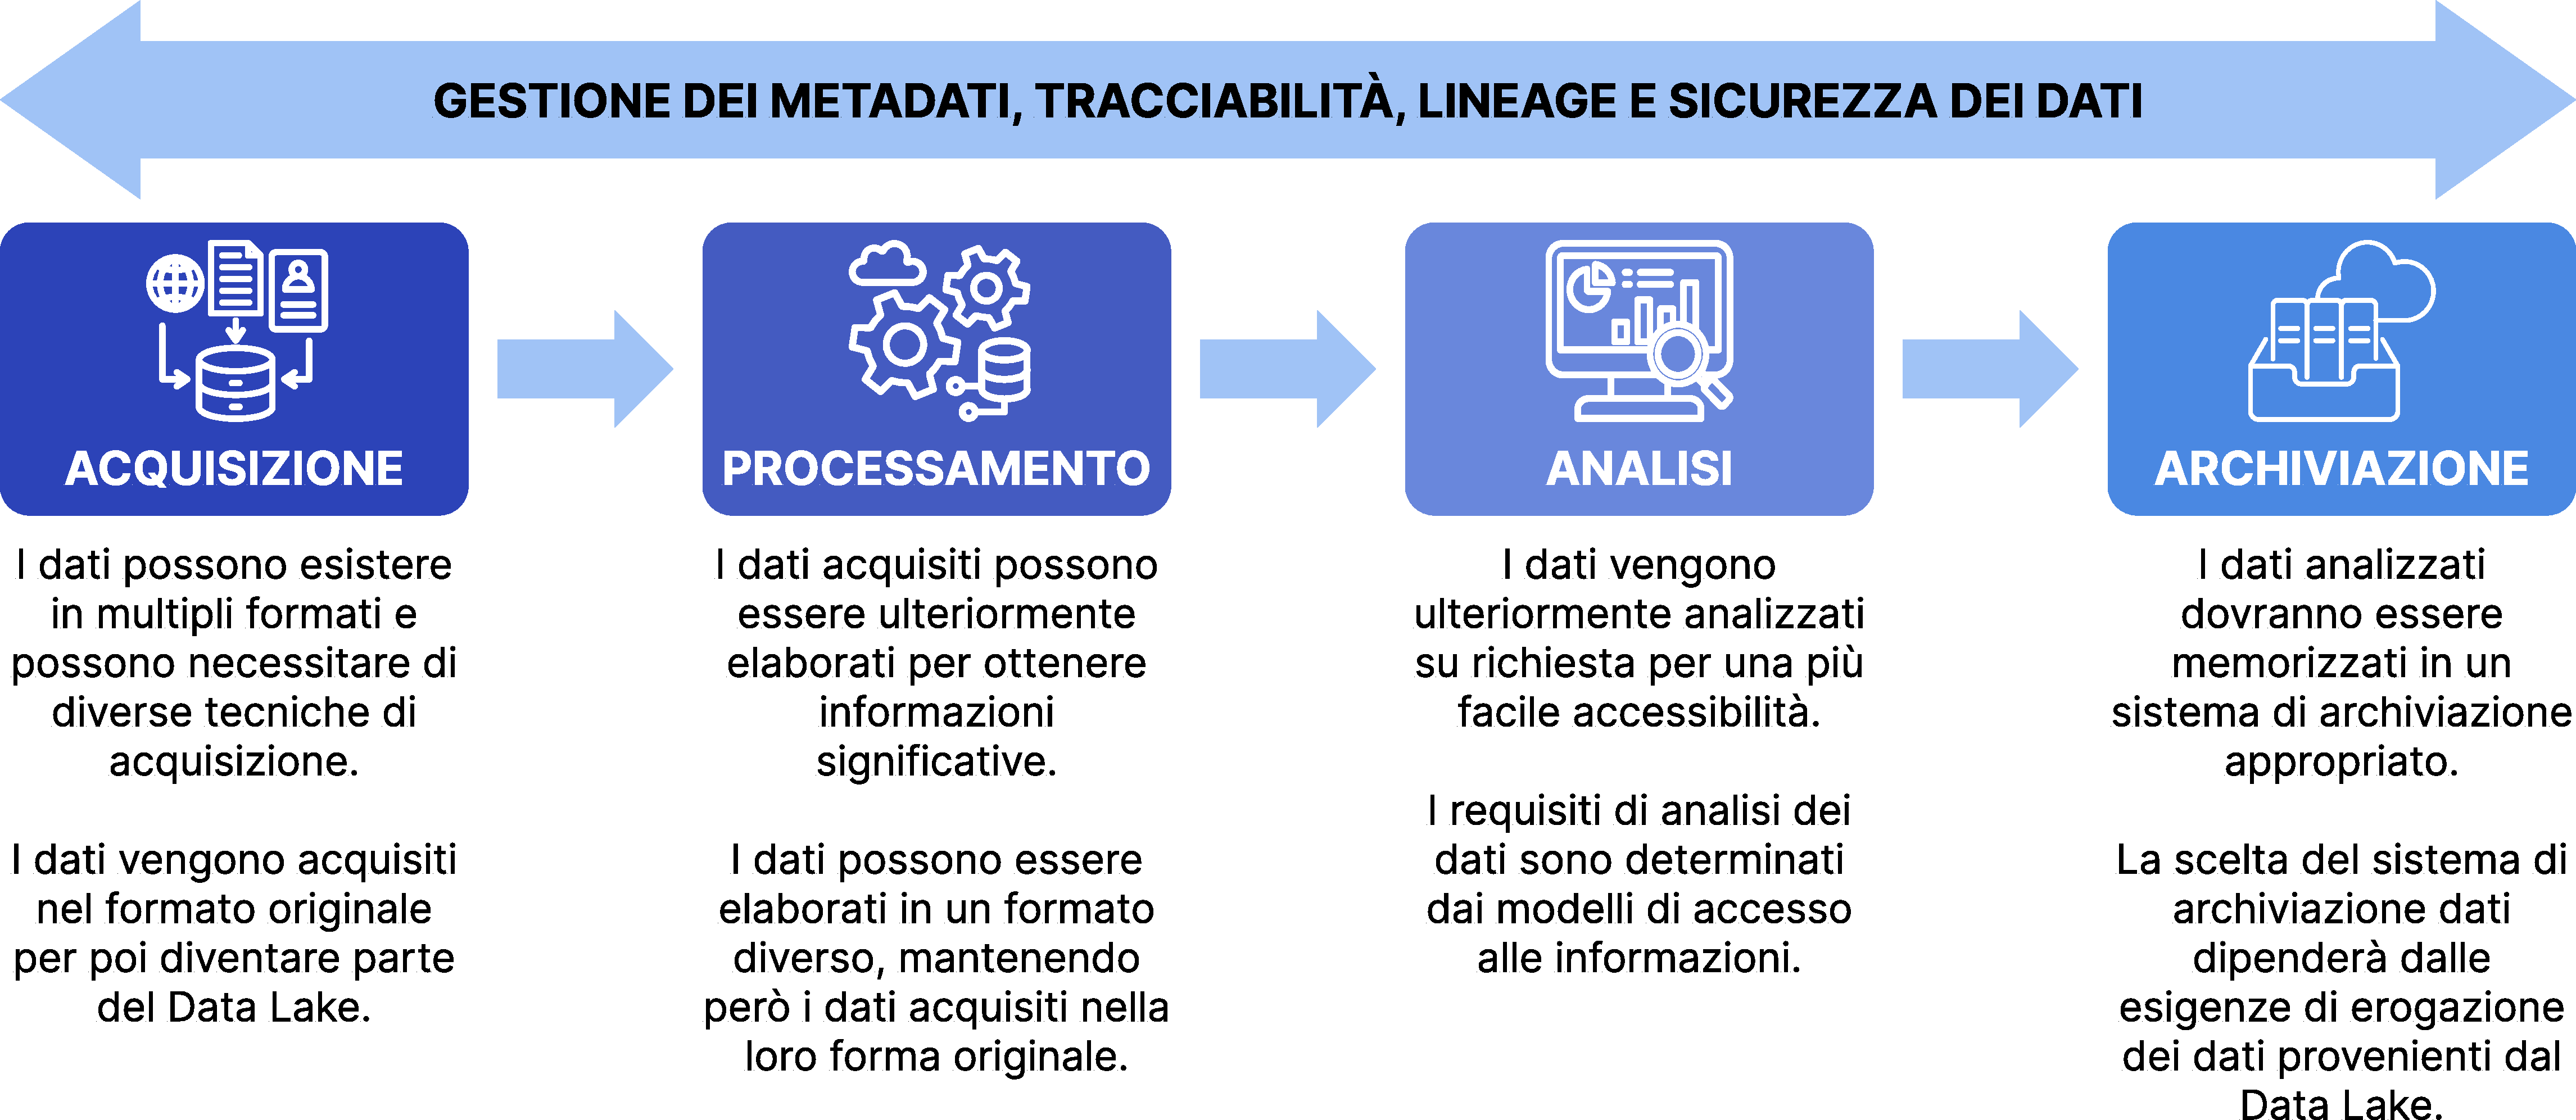
\includegraphics[width=0.75\linewidth]{figure//capitolo_3/Data Lake Life Cycle.png}
    \caption{Ciclo di vita dei dati nei Data Lake}
    \label{fig:Data Lake Life Cycle}
\end{figure}
\end{comment}

Originariamente i data lake sono stati creati per sopperire all’incapacità dei data warehouse di gestire i volumi crescenti, la velocità e l’ampia serie di Big Data. I data lake, anche se più lenti dei DW, sono più economici poiché non necessitano delle operazioni di trasformazione. Data la mancanza di necessità di definire degli obiettivi di business da applicare sui dati, hanno tantissimi possibili casi di utilizzo. Tuttavia, i due principali casi di utilizzo comprendono l’esplorazione della data science e le attività di ripristino e backup dei dati.\cite{ibm_data_architecture}

Di seguito è riportata una tabella riepilogativa che spiega le differenze tra un data lake e un data warehouse.\cite{aws_data_lake_vs_data_warehouse}

\begin{comment}
\begin{table}
    \centering
    \begin{tabular}{ccc}
        Caratteristiche & Data Lake & Data Warehouse\\
        Dati & Tutti i dati, compresi strutturati, non strutturati e semi-strutturati. & Dati relazionali da sistemi transazionali, database e applicazioni aziendali.\\
        Schema & Creato al momento dell’analisi. & Spesso progettato prima dell’implementazione, ma può essere creato anche al momento dell’analisi.\\
        Prezzo/Prestazioni & I risultati delle query diventano più veloci utilizzando l’archiviazione a basso costo e il disaccoppiamento dei processi di elaborazione e archiviazione. & Risultati delle query più rapidi utilizzando uno storage locale.\\
        Qualità dei dati & Qualsiasi dato curato e non. & Dati estremamente curati che fungono da versione veritiera centrale.\\
        Utenti & Analisti aziendali, data scientist, sviluppatori ed ingegneri di dati. & Analisti aziendali, data scientist e sviluppatori di dati.\\
        Analisi & Machine learning, analisi esplorativa, rilevamento di dati, streaming, analisi operativa, Big Data e profilazione. & Reporting in batch, BI e visualizzazioni.\\
    \end{tabular}
    \caption{Data Lake e Data Warehouse a confronto}
    \label{tab:data_lake_vs_data_warehouse}
\end{table}
\end{comment}

\subsection{I Data Fabric}
Secondo lo studio svolto dalla piattaforma Flexera\cite{flexera_cloud_computing} le aziende al giorno d’oggi adoperano un approccio ibrido e multi-cloud per l’archiviazione dei dati. L’87\% degli intervistati ha dichiarato di avere una strategia multi-cloud, mentre il 72\% sta adottando un approccio ibrido combinando l’uso di cloud pubblici e privati. Questa frammentarietà comporta una maggiore complessità nell’operazione di recupero e gestione dei dati. Tuttavia, secondo Mark Beyer, vice presidente analista di Gartner, «Il concetto di design emergente chiamato “data fabric” può essere una solida soluzione alle sfide sempre presenti nella gestione dei dati».\cite{gartner_data_fabric_architecture}
Non a caso Gartner espone la seguente definizione «Un data fabric è un progetto emergente di gestione dei dati per ottenere pipeline di integrazione dei dati, servizi e semantica flessibili, riutilizzabili e aumentati. Un data fabric supporta casi d'uso sia operativi che analitici, distribuiti su più piattaforme e processi di distribuzione e orchestrazione.»\cite{gartner_data_fabric}

I data fabric raccolgono i dati da sistemi legacy, data lake, data warehouse, database sql e app, fornendo una visione totalitaria delle prestazioni della compagnia. A differenza di questi singoli sistemi di storage dati, punta a creare una maggiore fluidità tra gli ambienti di dati cercando di risolvere il problema della complessità dei dati. Un data fabric elimina le complessità tecnologiche interessate dalle operazioni di trasferimento, trasformazione e integrazione dei dati, rendendo tutti i dati disponibili per l’intera azienda.\cite{ibm_data_fabric}

Per un data fabric non è necessario centralizzare i dati, ma l’importante è ordinare i componenti dove questi risiedono. Perciò, invece di sostituire o ricostruire l’infrastruttura esistente, per la creazione di un data fabric si aggiunge un nuovo livello di astrazione in cima alle fonti di dati sottostanti, consentendo agli utenti finali di accedere e gestire le informazioni di cui hanno bisogno senza che queste vengano duplicate in multiple aree di memoria. Un data fabric è un approccio progettuale che sfrutta i principi della visualizzazione dati, applicando tecniche di intelligenza artificiale e machine learning per semplificare le integrazioni dei dati, aumentarne l’affidabilità e la riutilizzabilità, oltre a fornire sistemi di analisi self-service.\cite{altexsoft_data_fabric}

\begin{comment}
\begin{figure}
    \centering
    \includegraphics[width=0.75\linewidth]{figure//capitolo_3/Data Fabric Architecture.png}
    \caption{Architettura di un Data Fabric}
    \label{fig:Data Fabric Architecture}
\end{figure}
\end{comment}

\subsubsection{Funzionalità chiave}

A questo punto è possibile riassumere le funzionalità principali di un’architettura data fabric come:\cite{gft_data_fabric}
\begin{itemize}
    \item Combinare dati provenienti da sistemi, software e fonti differenti in un unico ambiente che non sia obbligatoriamente centralizzato, ma gestito e accessibile come un unico sistema.
    \item Garantire alte prestazioni in termini di velocità, capacità, scalabilità e affidabilità per soddisfare ogni eventuale necessità.
    \item Supportare ambienti distribuiti su larga scala.
    \item Garantire una gestione attiva dei metadati.
    \item Fornire funzionalità di Data Governance integrata.
    \item Automatizzare i task ripetitivi.
\end{itemize}

\subsection{Il modello multidimensionale dei dati}

Secondo diversi studi è emerso che i modelli di dati tradizionali, come il modello E-R e il modello relazionale, non forniscono un buon supporto ai sistemi appositi per la gestione di dati a fini analitici. Per sopperire a tale problematica, nel tempo sono emersi differenti modelli dai dati basati su una visione multidimensionale dei dati in questione. Questi modelli multidimensionali categorizzano i dati come \textit{fatti} (anche definiti come “misure”) o \textit{dimensioni}.\cite{ieee_multidimensional_data_modeling}

Il \textbf{modello multidimensionale} deriva la sua idea dalla constatazione che gli oggetti che influenzano il processo decisionale sono \textit{fatti} che accadono nel mondo aziendale ed ogni occorrenza di un fatto corrisponde ad un evento accaduto. Inoltre, per ognuno dei fatti registrati si è interessati ai valori di insiemi di \textit{misure} o \textit{metriche} che descrivono quantitativamente gli eventi in questione. Poiché gli eventi da registrare sono moltissimi viene adoperato un modello che permette di selezionarli e raggrupparli come se fossero collocati all’interno di uno spazio n-dimensionale i cui assi, definiti come \textit{dimensioni} di analisi, determinano diverse prospettive per la loro identificazione.\cite{unibo_introduzione_al_data_warehousing}

\subsubsection{Il cubo multidimensionale}

I database che sfruttano il modello multidimensionale considerano i dati come cubi che generalizzano i fogli di calcolo a qualsiasi numero di dimensioni. Inoltre, i cubi supportano gerarchie nelle dimensioni e misure senza duplicare le loro definizioni. Una raccolta di cubi correlati costituisce un database multidimensionale oppure un data warehouse. Sebbene l’immagine associabile all’idea del cubo sia di sole tre dimensioni, in realtà un cubo può teoricamente avere un numero indefinito di dimensio ni, per quanto l’aumentare di dimensioni comporti la necessità di sistemi appositi per poterli gestire.\cite{researchgate_multidimensional_db}

Più precisamente in un cubo le dimensioni definiscono la struttura del cubo utilizzata per effettuare le sezioni che lo compongono, mentre le misure forniscono valori numerici aggregati che siano utili all’utente finale. Un cubo consente ad un’applicazione di recuperare i valori delle misure come se queste si trovassero nelle celle del cubo, dove quest’ultime vengono definite per ogni possibile valore riepilogativo. In altre parole, una cella è definita dall’intersezione degli elementi sull’asse delle dimensioni e contiene i valori aggregati delle misure che corrispondono a quella specifica intersezione.\cite{microsoft_multidimensional_models}

\begin{comment}
\begin{figure}
    \centering
    \includegraphics[width=0.75\linewidth]{figure//capitolo_3/Multidimensional Data Cube.png}
    \caption{Rappresentazione di dati Multidimensionali sottoforma di cubo}
    \label{fig:Multidimensional Data Cube}
\end{figure}
\end{comment}

Per semplificare il concetto, una tabella di un database è strutturata come un foglio di calcolo e memorizza i singoli record in un formato bidimensionale, riga per colonna; ogni fatto corrisponde all’intersezione di due dimensioni, una riga e una colonna. Invece, un cubo multidimensionale estende la singola tabella con livelli ulteriori aggiungendo una dimensione per ogni livello permettendo di rappresentare in questo modo maggiori informazioni per un singolo evento.\cite{ibm_multidimensional_data}

\subsection{Database OLTP e OLAP}

I database relazionali sono stati uno dei punti cardine delle infrastrutture delle applicazioni aziendali per più di venti anni. Con l’avanzare della tecnologia si pose l’obiettivo di fornire alle compagnie un sistema di gestione delle informazioni che coprisse tutti gli ambiti principali che vanno dalla pianificazione dei processi aziendali fino alle analisi individuali; tuttavia, ciò non è stato possibile. Più complessi diventano i requisiti aziendali e maggiore è stato il focus sul migliorare l’elaborazione transazionale, creando appositi database che prendono il nome di sistemi \textbf{OLTP} (\textit{On-Line Transactional Processing}, \textit{elaborazione transazionale on-line}). Ciò ha comportato la necessità di spostare le applicazioni di ambito analitico e finanziario in sistemi separati ad hoc che avessero maggiore flessibilità e prestazioni, questi prendono il nome di sistemi \textbf{OLAP} (\textit{On-Line Analytical Processing}, \textit{elaborazione analitica on-line}). Entrambi i sistemi sono basati sulla teoria relazionale dei dati, ma utilizzano approcci tecnici differenti. Inoltre, l’OLTP è il prerequisito necessario per l’OLAP, ma solo con l’OLAP le aziende possono comprendere al meglio i dati generati dal proprio lavoro e trarre delle conclusioni che permettano di migliorarlo.\cite{scribd_oltp_olap}

I sistemi OLTP sono strutture progettate per alti volumi di query con accesso specifico con l’obiettivo di massimizzare l’efficienza di queste operazioni, mentre i sistemi OLAP utilizzano tecnologie di archiviazione dei dati per supportare l’analisi e l’estrazione di dati storici a lungo termine per fornire agli analisti dei report da cui ricavare informazioni per prendere decisioni aziendali.\cite{ieee_oltp_olap}
Per comprendere meglio questo discorso di seguito vengono spiegati i concetti di OLAP e OLTP, in modo da poter approfondire l’argomento.

\begin{itemize}
    \item \textit{OLTP}. Questi database in genere comprendono dati transazionali, ovvero informazioni che tengono traccia delle informazioni correlate alle attività di un’azienda. Tali transazioni devono essere atomiche\footnote{Un'operazione si definisce \textit{atomica} se questa ha sempre un esito o positivo o negativo, non può rimanere in uno stato parziale.} e coerenti. Tali sistemi sono progettati per elaborare e archiviare in modo efficiente singole transazioni, permettendo in questo modo di gestire grandi quantità di transazioni in modo indipendente.\cite{microsoft_oltp}
    \item \textit{OLAP}. È una tecnologia che consente di organizzare i database aziendali di grandi dimensioni e supporta l’esecuzione di analisi complesse. Può essere usata per seguire query di analisi complesse senza influire negativamente sui sistemi transazionali. Poiché i database utilizzati dalle aziende, principalmente OLTP, non sono progettati per sopperire a necessità di analisi, il recupero delle informazioni da questi sistemi è un compito esoso si in termini di tempo che di prestazioni. A questo scopo sono stati ideati i database OLAP, ottimizzati appositamente per gestire intensi carichi di lavoro in lettura e ridotti in scrittura.\cite{microsoft_olap}
\end{itemize}

Di seguito è riportata una tabella riepilogativa che spiega le differenze tra un database OLAP e uno OLTP.\cite{aws_oltp_vs_olap}

\begin{comment}
\begin{table}
    \centering
    \begin{tabular}{ccc}
        Criteri & OLAP & OLTP\\
        Scopo & Aiuta ad analizzare grandi volumi di dati per supportare il processo decisionale. & Consente di gestire ed elaborare transazioni in tempo reale.\\
        Origine dati & Utilizza dati storici e aggregati provenienti da diverse origini. & Utilizza transazioni in tempo reale provenienti da un’unica origine.\\
        Struttura dei dati & Adopera database multidimensionali (cubi) oppure database relazionali. & Adopera solo database relazioni.\\
        Modello dei dati & Utilizza lo schema a stella, a fiocco di neve oppure altri modelli analitici. & Utilizza modelli normalizzati o denormalizzati.\\
        Volume dei dati & Ha requisiti di archiviazione elevati (TB o PB). & Ha requisiti di archiviazione inferiori (GB).\\
        Tempo di risposta & Ha tempi di risposta più lunghi (s o m). & Tempi di risposta brevi (ms).\\
    \end{tabular}
    \caption{Differenze tra database OLTP e OLAP}
    \label{tab:oltp_vs_olap}
\end{table}
\end{comment}

\subsection{Schema dei database}

In precedenza è stato affermato che uno dei componenti più importanti per la gestione dei dati sono i database, che possono avere diversi formati, utilizzi e specializzazioni. Tuttavia, bisogna però fare anche una precisazione, ovvero che nel mondo della gestione dei dati, uno strumento importante se non essenziale per la strutturazione e l’organizzazione dei dati all’interno di un database di un data warehouse è il suo relativo schema.

Uno schema di database rappresenta la configurazione logica di tutto o parte di un database relazionale. Esso corrisponde sia ad una rappresentazione visiva sia all’insieme di regole applicate per la strutturazione del database a cui fa riferimento. In un dizionario di dati, uno schema di database indica come le entità (tabelle, viste, procedure, eccetera) compongono quest’ultimo si relazionano tra loro.  Esistono due differenti schema di database, ovvero: \textbf{Schema a stella} (o \textit{Star schema}) e \textbf{Schema a fiocco di neve} (o \textit{Snowflake schema}).\cite{researchgate_database_schemas}
\begin{comment}
\begin{table}[!h]
    \centering
    \begin{tabular}{ccc}
         \textbf{Caratteristica} & \textbf{Star Schema} & \textbf{Snowflake Schema}\\
         Descrizione & Come suggerisce il nome, tale schema prende la forma di una stella, dove la tabella dei fatti si trova al centro dello schema, mentre le varie tabelle delle dimensioni si trovano agli estremi. La tabella dei fatti contiene al suo interno, oltre ai propri valori, le chiavi esterne che fanno riferimento le chiavi primarie presenti nelle tabelle delle dimensioni. & Anche in questo caso, il suo nome deriva dalla sua conformazione. Questo schema è composto da tre differenti tipi di tabelle, ovvero dei fatti, delle dimensioni e delle sub-dimensioni. Il funzionamento della tabella dei fatti è simile allo schema a stella, in quanto contiene le chiavi esterne per collegarsi alle chiavi primarie delle tabelle delle dimensioni, che possono essere collegate a loro volta con altre tabelle dalle dimensioni normalizzate (sub-dimensioni). Data questa struttura, in questo schema viene introdotto il principio della gerarchia.\\
    %      Design & 
    % \begin{figure}
    %     \includegraphics[width=0.5\linewidth]{figure//capitolo_3/DW - Star schema.jpg}
    %     \label{fig:Star schema}
    % \end{figure} & 
    % \begin{figure}
    %     \centering
    %     \includegraphics[width=0.5\linewidth]{figure//capitolo_3/DW - Snowflake schema.jpg}
    %     \label{fig:Snowflake schema}
    % \end{figure}\\
    \end{tabular}
    \caption{Schema dei database a paragone}
    \label{tab:database_schemas}
\end{table}
\end{comment}

\section{La conoscenza}

Per migliaia di anni gli esseri umani hanno discusso sul significato di “\textit{conoscenza}”, su cosa significhi conoscere qualcosa e su come le persone possano generare e condividere nuova conoscenza. Nonostante l’importanza di tale dilemma nelle discussioni affrontate nel corso della storia, solo negli ultimi anni il mondo del business ha iniziato a riconoscere l’importanza della conoscenza come una risorsa.\cite{knowledge_management_tools}
La crescente evoluzione del mondo del Data Warehousing e dei Big Data ha portato alla necessità di svolgere studi, generare teorie o modelli e progettare strumenti che potessero aiutare le persone nell’estrazione di informazioni, ritenute, utili. Questa branca del mondo digitale prende il nome di \textbf{Knowledge Discovery in Databases} (\textit{KDD}), ovvero \textit{scoperta della conoscenza dei database}.

\subsection{La piramide della conoscenza}
Finora abbiamo parlato del mondo dell’analisi dei dati dando per scontato il concetto del legame tra i dati e la conoscenza, per quanto sia stata esplicitata più volta la loro rilevanza. «Tipicamente l'informazione è definita in termini di dati, la conoscenza in termini di informazione e la saggezza in termini di conoscenza», queste sono le parole della giornalista Jennifer Rowley\cite{rowley_dikw_hierarchy}, che permettono di descrivere brevemente la rappresentazione della \textit{piramide della conoscenz}a, meglio conosciuta come \textbf{DIKW pyramid} (\textit{Data, Information, Kownledge and Windsome pyramid}), ovvero il modello creato per spiegare il processo di trasformazione dei dati e di come essi possano acquistare effettivamente, trasformandosi in informazione, conoscenza e saggezza.

\begin{comment}
\begin{figure}
    \centering
    \includegraphics[width=0.75\linewidth]{figure//capitolo_3/DIKW Pyramid.png}
    \caption{Piramide della conoscenza}
    \label{fig:DIKW Pyramid}
\end{figure}
\end{comment}

L’origine della piramide DIKW è incerta, è ignoto sia chi sia quando sia stata creata, come meglio spiegato dal professor Danny P. Wallace\cite{knowledge_management_historical}
«La presentazione delle relazioni tra dati, informazioni, conoscenza e talvolta saggezza in una disposizione gerarchica fa parte del linguaggio della scienza dell’informazione da molti anni. Sebbene non sia chiaro quando e da chi tali relazioni siano state presentate per la prima volta come gerarchia, l’ubiquità della nozione di gerarchia è incorporato nell’uso dell’acronimo DIKW come rappresentazione abbreviata della trasformazione da dati a informazione a conoscenza in saggezza».

Per comprendere meglio tale rappresentazione, è meglio approfondire ognuno dei suoi elementi:\cite{researchgate_revising_dikw_pyramid}
\begin{enumerate}
    \item \textbf{Data} (\textit{Dati}). I dati sono solitamente definiti come fatti e statistiche che vengono ricavati insieme per svolgere riferimenti o analisi. I dati generalmente vengono combinati, ricombinati, confezionati, venduti, e ridistribuiti, proprio per questo motivo sono soggetti ad un uso improprio, quasi abuso. Inoltre, bisogna sempre ricordare che la raccolta di dati, anche in ordine di peta, exa o zettabyte, non ha alcun valore se essi possono essere inaccurati, obsoleti oppure intenzionalmente o non falsi. Proprio per questo motivo, i dati non portano sempre delle direttamente informazioni, ed è impossibile concludere che il volume di dati raccolto e archiviato per creare “informazioni” stiano effettivamente creando maggiori o migliori informazioni. È quindi possibile definire che i dati sono fondamentali perché il percorso verso le informazioni, la conoscenza e la saggezza si basa su di loro, tuttavia sono anche definibili inutili poiché da soli non hanno alcun valore.
    \item \textbf{Information} (\textit{Informazione}). Le informazioni, in termini generali, sono comunemente definite come fatti forniti o appresi su qualcosa o qualcuno. Nell’ambito digitale, l’informazione può essere definita come il significato attribuito dagli esseri umani ai dati raccolti o a sottoinsiemi selezionati di dati, tipicamente accompagnato da una presunzione di verità o di fatto. Pertanto, i dati interrogati possono diventare informazioni, ma se l’informazione sia utile o preziosa dipende interamente dal mondo di interrogazione dell’accuratezza dei dati sottostanti. Come espresso in precedenza, le informazioni possono definirsi valide solamente quando la fonte da cui provengono è valida, poiché altrimenti produrranno risultati errati. Ad aumentare l’importanza del valore delle informazioni vi è l’imprescindibile regola per cui per ottenere informazioni valide e utili dai dati è necessario svolgere le domande nel giusto modo e forma. La sbagliata interpretazione delle informazioni è uno scenario molto comune poiché è probabile che accada facilmente. Considerando quanto detto, l’informazione non porta necessariamente alla conoscenza e maggiori informazioni, per quanto corrette, non aumentano sempre la conoscenza. Pertanto, l’informazione potrebbe diventare conoscenza, ma non inevitabilmente o perlomeno non utile.
    \item \textbf{Knowledge} (\textit{Conoscenza}). La conoscenza è generalmente definita come fatti, informazioni e competenze apprese attraverso l’esperienza o l’istruzione. Data questa definizione, per quanto corretta, necessita di una precisazione, ovvero è possibile acquisire conoscenza su un argomento attraverso la raccolta di informazioni e le esperienze di vita, ma la conoscenza su un argomento non implica automaticamente la conoscenza su altri argomenti, anche se affini; per questo motivo il processo di acquisizione della conoscenza deve essere ripetuto su ogni argomento. In termini generali, maggiore è la conoscenza di una persona e più è probabile che soddisfi più bisogni umani e che ottenga ulteriore successo nella vita. Conoscenza e saggezza sono strettamente correlate, ma la saggezza comprende sia un volume più ampio che una maggiore durata di conoscenza accumulata.
    \item \textbf{Wisdom} (\textit{Saggezza}). La saggezza è comunemente definita come la qualità di avere esperienza, conoscenza e buon giudizio. A questa definizione si potrebbe aggiungere l’aggettivo “estesa”, poiché quantità limitate di questi elementi non sono sufficienti per creare saggezza. La saggezza si crea attraverso l’informazione, l’esperienza e la conoscenza, oltre all’apporto umano di analisi ed estrapolazione. L’uso intelligente dell’informazione, dell’esperienza e della conoscenza è vitale per la saggezza.
\end{enumerate}

\subsection{Tipologie di conoscenza}

Parlare in termini generici di conoscenza non è sbagliato, tuttavia, sarebbe sicuramente più corretto fare un approfondimento sulle varie categorie in cui la conoscenza può essere suddivisa.\cite{getguru_types_of_knowledge}

\begin{itemize}
    \item \textit{Conoscenza esplicita}. È la conoscenza che riguarda gli argomenti che sono facilmente documentabili in modo sistematico e condivisibili su larga scala (si tratta di documentazione che può essere adoperata per svolgere un lavoro, prendere una decisone o interagire con una fascia di utenza).
    \item \textit{Conoscenza implicita}. È la conoscenza acquisita con la messa in pratica. È possibile acquisirla applicando in una situazione specifica la conoscenza esplicita. Questo tipo di conoscenza è solitamente esculo dalle conoscenze di base formali, poiché può essere molto difficile da documentare e ricavare.
    \item \textit{Conoscenza tacita}. È la conoscenza di tipo intangibile che può essere difficile da spiegare in modo diretto. Questo tipo di conoscenza è informale e viene appresa con l’esperienza nel tempo e solitamente si applica ad una specifica situazione. 
    \item \textit{Conoscenza dichiarativa}. È la conoscenza che si riferisce a informazioni statiche e fatti specifici, di facile accesso, su un determinato argomento. Questa è un tipo di conoscenza in cui l’individuo che la mette in atto è consapevole in modo cosciente della propria comprensione della materia.
    \item \textit{Conoscenza procedurale}. È la conoscenza che si focalizza sul come funzionano determinate cose e viene dimostrata attraverso la capacità di fare qualcosa. Mentre la conoscenza dichiarativa si concentra maggiormente su “chi, cosa, dove o quando”, tale conoscenza è meno articolata ed è dimostrata attraverso l’azione o documentata attraverso specifici manuali.
    \item \textit{Conoscenza a posteriori}. È la conoscenza che rappresenta la soggettività acquisita dall’esperienza individuale. Per quanto non debba essere documentata, svolge un ruolo di rilevante importanza nell’essere applicata in determinate situazioni. Permette agli individui di avere una presa di coscienza da parte per riconoscere i propri punti di forza e debolezza derivati dalle proprie esperienze passate.
    \item \textit{Conoscenza a priori}. È la conoscenza acquisita indipendentemente dall’esperienza o dalle prove. Questo tipo di conoscenza viene spesso condivisa attraverso il ragionamento logico o la capacità di pensare in modo astratto.
\end{itemize}

\subsection{Gestione della conoscenza}

La \textbf{gestione della conoscenza} (\textit{GC}, o \textit{Knowledge Management – KM}) aziendale implica la gestione formale delle risorse di conoscenza per facilitarne l’accesso e il riutilizzo, generalmente adoperando tecnologie informatiche avanzate. Il KM viene definito formale in quanto la conoscenza viene classificata e categorizzata in base ad un’ontologia\footnote{L'\textit{ontologia} è lo studio dell'essere in quanto tale, nonché delle sue categorie fondamentali.\cite{wikipedia_ontologia}} prestabilita (che però è in continua evoluzione), in dati strutturati e semi-strutturati e in basi di conoscenza.\cite{overview_of_knowledge_management}

In altri termini, la gestione della conoscenza riguarda l’utilizzo della capacità intellettuale di un’organizzazione in modo sistematico e organizzato al fine di ottenere efficienze, garantire un vantaggio competitivo e stimolare l’innovazione.\cite{ieee_enterprise_knowledge_management}

Per essere più precisi è possibile fare riferimento alla definizione data da Gartner, ovvero: «La gestione della conoscenza è un processo aziendale che formalizza la gestione e l’utilizzo del patrimonio intellettuale di un’impresa. La KM promuove un approccio collaborativo e integrativo alla creazione, acquisizione, organizzazione, accesso e utilizzo delle risorse informative, inclusa la conoscenza tacita e non catturata delle persone».\cite{gartner_knowledge_management}

\subsubsection{Fasi della gestione della conoscenza}

È possibile definire che tale procedimento si componga di quattro fasi principali, ovvero:\cite{knowledge_management_process}
\begin{enumerate}
    \item \textit{Acquisizione}. Tale fase corrisponde al processo organizzativo interno all’azienda che permette di facilitare la creazione della conoscenza tacita ed esplicita, partendo dalle persone della compagnia e integrando il livello organizzativo, associando il processo di identificazione di informazioni che creino una conoscenza proveniente dall’esterno.
    \item \textit{Archiviazione}. Tale fase corrisponde al processo di salvataggio delle conoscenze acquisite nella fase precedente all’interno di un apposito sistema che permetta di svolgere un’archiviazione di tale conoscenza in modo organizzato. Questa fase implica un processo di conversione che comporta organizzazione, strutturazione, archiviazione e combinazione della conoscenza al fine di facilitarne l’uso da parte degli utenti finali che dovranno necessitarne.
    \item \textit{Distribuzione}. Tale fase corrisponde al processo di condivisione delle informazioni salvate con l’obiettivo di portare alla creazione di nuove conoscenze derivanti dalle prime. Il solo possesso di conoscenza da parte di un’azienda non è di per sé sufficiente, quest’ultima dovrebbe garantire il flusso delle informazioni al fine di permettere un apprendimento tra gli individui, comportando un miglioramento delle prestazioni nel procedimento di gestione delle stesse. Il modo più efficace per diffondere la conoscenza è attraverso una metodologia che consenta un trasferimento sistematico.
    \item \textit{Utilizzo}. Tale fase corrisponde al processo di sfruttamento delle fasi precedenti per far sì che l’acquisizione della conoscenza possa essere utilizzata come base per lo sviluppo di nuove conoscenze attraverso l’integrazione, l’innovazione, la creazione e l’estensione della conoscenza pregressa. Per tale motivo, l’uso della conoscenza può definirsi tale quando attraverso esso vengono prese decisioni o apportate migliorie.
\end{enumerate}

\begin{comment}
\begin{figure}[!h]
    \centering
    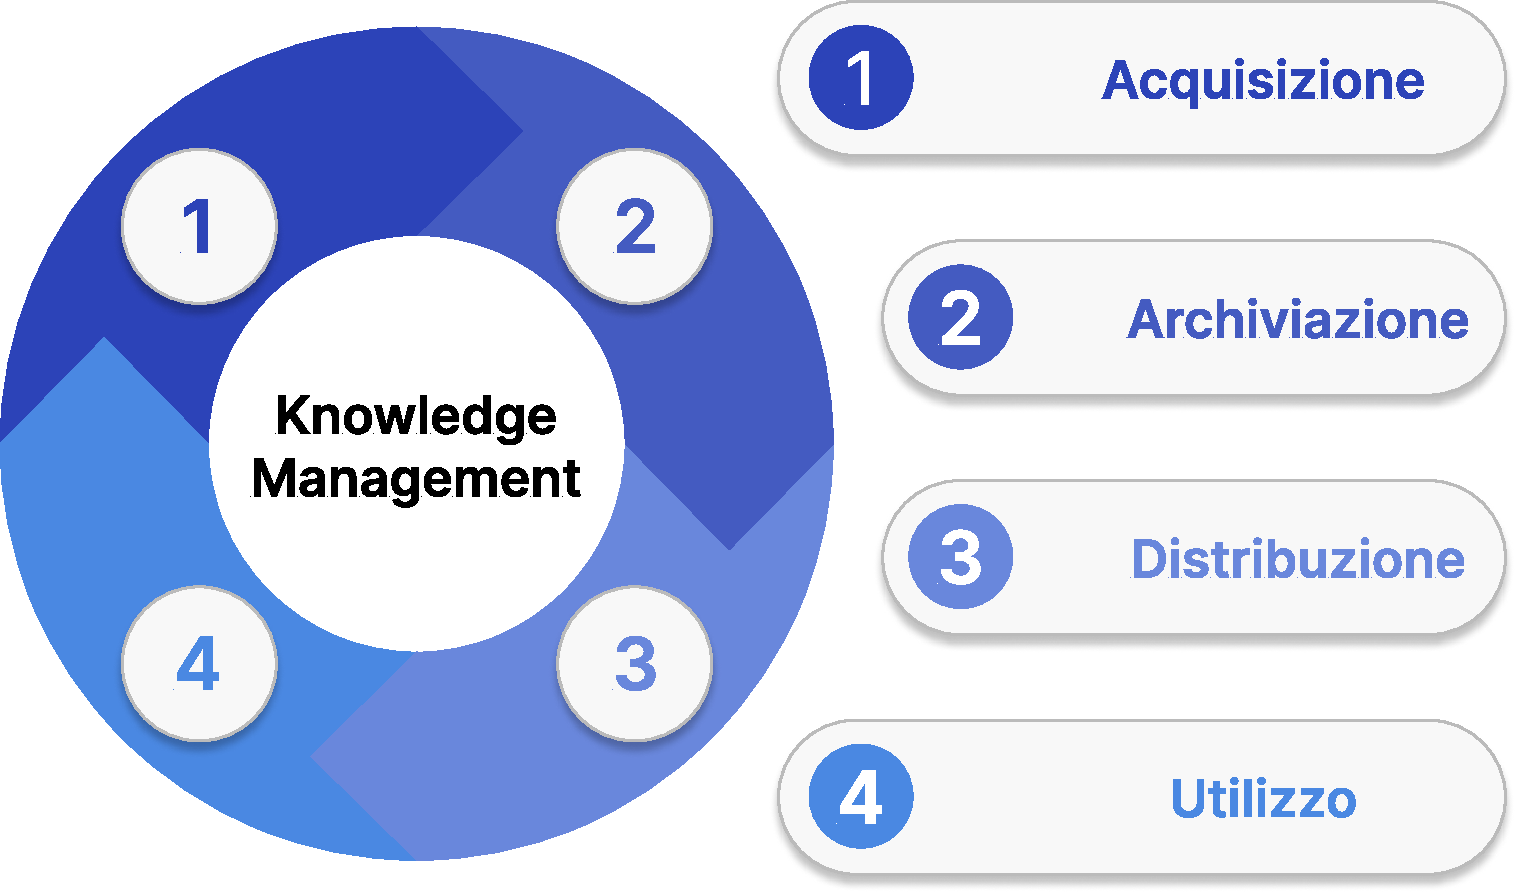
\includegraphics[width=0.5\linewidth]{figure//capitolo_3/Knowledge Management Process.png}
    \caption{Ciclo dell'informazione}
    \label{fig:Knowledge Management Process}
\end{figure}
\end{comment}

\subsubsection{Componenti della gestione della conoscenza}

Per svolgere tale gestione, naturalmente, sono necessarie delle componenti imprescindibili, più precisamente:\cite{knowledge_management_components}

\begin{itemize}
    \item \textit{Persone}. Tale componente fa riferimento a tutte le persone che partecipano alla gestione della conoscenza creando, condividendo e utilizzando tale conoscenza nei vari modi possibili. Una gestione efficace della conoscenza richiede un pensiero, pianificazione, innovazione ed esecuzione che possono essere raggiunti unicamente grazie al coinvolgimento umano. D'altronde le risorse umane sono considerate la principale ragione dietro il successo di qualsiasi impresa.
    \item \textit{Processo}. Tale componente fa rifermento alla metodologia, o più correttamente per l’appunto processo, che gli utenti adoperano per accedere alla conoscenza di cui necessitano. Come mostrato precedentemente il processo di gestione della conoscenza comprende diverse fasi e assicurarsi che l’intero flusso di lavoro sia efficiente è un punto di importanza critica.
    \item \textit{Tecnologia}. Tale componente fa riferimento alle infrastrutture e ai sistemi di supporto adoperati per svolgere il compito di gestione. L’obiettivo principale dell'utilizzo della tecnologia è supportare tutte le attività dell'intero procedimento, recupero, archiviazione, condivisione e sfruttamento.
    \item \textit{Strategia}. Tale componente fa riferimento alla pianificazione di tutte le attività svolte da un’azienda per applicare una gestione che permetta di sfruttare la conoscenza in modo adeguato ed efficiente. Inoltre, comprende la definizione degli obiettivi da raggiungere e la strada d    a perseguire per farlo.
\end{itemize}

\begin{comment}
\begin{figure}[!h]
    \centering
    \includegraphics[width=0.5\linewidth]{figure//capitolo_3/Knowledge Management Components.png}
    \caption{Elementi fondanti della gestione della conoscenza}
    \label{fig:Knowledge Management Components}
\end{figure}
\end{comment}

\subsection{Sistemi per la gestione della conoscenza}

Prima dell'avvento della tecnologia, la gestione della conoscenza avveniva attraverso canali di comunicazione analogici e la conservazione di tale conoscenza era lasciata alle biblioteche. Tuttavia, con l’evoluzione della scienza è stato possibile per l’uomo di disporre di strumenti tecnologici che potessero semplificare tale compito, comportando cambiamenti non solo nel sistema di archiviazione ma anche nelle metodologie da applicare per svolgere tale compito. A questo scopo sono nati degli applicativi che permettessero di supportare le fasi del ciclo dell’informazione e della sua gestione.

Più precisamente, un \textbf{sistema di gestione della conoscenza} (\textit{Knowledge Management System, KMS}) sfrutta la conoscenza collettiva dell’azienda per portare migliori efficienze operative. Tali sistemi sono supportati dall’utilizzo di una conoscenza di base. Di solito sono fondamentali per una gestione efficiente ed efficace della conoscenza in questione, creando un ambiente centralizzato per memorizzare le informazioni e accedervi velocemente secondo le necessità del caso.\cite{ibm_knowledge_management}

\subsection{Scoperta della conoscenza nei database (Knowledge Discovery in Databases)}

A livello astratto, il campo del KDD si occupa dello sviluppo di metodi e tecniche per dare senso ai dati. Il problema di base affrontato dal processo KDD consiste nel mappare dati a basso livello (che sono tipicamente troppo voluminosi per essere compresi e assimilati facilmente) in altre forme che potrebbero essere più compatte, più astratte o più utili. Al centro del processo c’è l’applicazione di specifici metodi di data mining per la scoperta e l’estrazione di pattern.\cite{from_data_mining_to_knowledge_discovery}

La frase “\textit{knowledge discovery in databases}” viene attribuita al data scientist Usama Fayyad a seguito di un workshop tenuto nel 1989, dove venne usata per esplicitare che il risultato finale dell’indagine sui dati dovrebbe essere la scoperta di conoscenze utilizzabili. La KDD comprende tutti i processi, automatizzati e non, che migliorano o consentono l’esplorazione di database (indipendentemente dalle loro dimensioni), per recuperare potenziali conoscenze.\cite{knowledge_discovery_in_databases}

\subsubsection{Il processo KDD}

Il processo KDD è di tipo iterativo e interattivo (dove molte delle decisioni sono dipendenti dalle scelte dell’utente) e coinvolge nove differenti fasi, ovvero:\cite{researchgate_data_mining_and_knowledge}

\begin{enumerate}
    \item \textit{Apprendimento del dominio dell’applicazione} (). Questa fase comprende lo sviluppo della comprensione delle conoscenze pregresse pertinenti e degli obiettivi dell’applicazione.
    \item \textit{Creazione di un set di dati target}. Questa fase include la selezione di un set di dati o la focalizzazione su un sottoinsieme di dati su cui bisogna effettuare la scoperta della conoscenza.
    \item \textit{Pulizia e pre-elaborazione dei dati}. Questa fase svolge le operazioni di base per la pulizia dei dati, la raccolta di informazioni utili alla modellazione, la definizione di regole per la gestione dei campi mancanti e la gestione del database.
    \item \textit{Riduzione e proiezione dei dati}. Questa fase comprende la ricerca di caratteristiche utili per rappresentare i dati e l’uso di metodi per la diminuzione delle dimensioni o del numero di variabili da prendere in considerazione.
    \item \textit{Scelta della funzione di data mining}. Questa fase si occupa di decidere lo scopo del modello derivato dall’applicazione dell’algoritmo di data mining.
    Scelta dell’algoritmo di data mining. Questa fase include la selezione dei metodi da adoperare per cercare modelli nei dati.
    \item \textit{Data mining}. Questa fase effettua la ricerca dei modelli di interesse in una particolare forma di rappresentazione o in un insieme di tali rappresentazioni.
    \item \textit{Interpretazione}. Queta fase comprende l’interpretazione dei modelli scoperti dalla fase precedente e, se necessario, la riapplicazione di alcune delle fasi già svolte.
    \item \textit{Utilizzo della conoscenza scoperta}. Questa fase include l’integrazione della conoscenza appresa nel sistema di performance, intraprendendo azioni basate s tale conoscenza o semplicemente documentarla.
\end{enumerate}

In generale è possibile raggruppare queste fasi in cinque passaggi essenziali che permettono di descrivere a pieno il processo KDD, ovvero:\cite{knowledge_science}:

\begin{enumerate}
    \item \textit{Comprendere il dominio dell’applicazione per formulare il problema}. Questo è chiaramente il prerequisito per recuperare informazioni utili e scegliere dei metodi appropriati di apprendimento automatico ed estrazione dati, dipendentemente dallo scopo finale dell’applicazione e dalla natura dei dati di origine.
    \item \textit{Raccolta e pre-elaborazione dei dati}. Questo passaggio comprende la selezione delle fonti dati, la rimozione di eventuali rumori e anomalie, la gestione di eventuali dati mancanti, la trasformazione e la riduzione del volume di dati. Date queste numerose operazioni, questo è il passaggio che richiede maggior tempo nell’intero processo.
    \item \textit{Data mining}. Questo passaggio è necessario per l’estrazione dei modelli o pattern nascosti dei dati.
    \item \textit{Interpretazione (o post-elaborazione) dei dati}. Questo passaggio si occupa di interpretare la conoscenza scoperta mediante l’uso dei metodi di natura induttiva. Gli esperimenti mostrano che i pattern o i modelli scoperti dai dati non sono sempre di interesse o utilizzo diretto, e il processo di KDD è necessariamente iterativo con la valutazione della conoscenza scoperta.
    \item \textit{Applicazione delle conoscenze}. In alcuni casi, non è necessario adoperare sistemi informativi per sfruttare la conoscenza scoperta, mentre in altri casi l’utente può aspettarsi che questa possa essere inserita nei propri dispositivi di analisi per essere messa a disposizione di diversi programmi.
\end{enumerate}

\begin{comment}
\begin{figure}[!h]
    \centering
    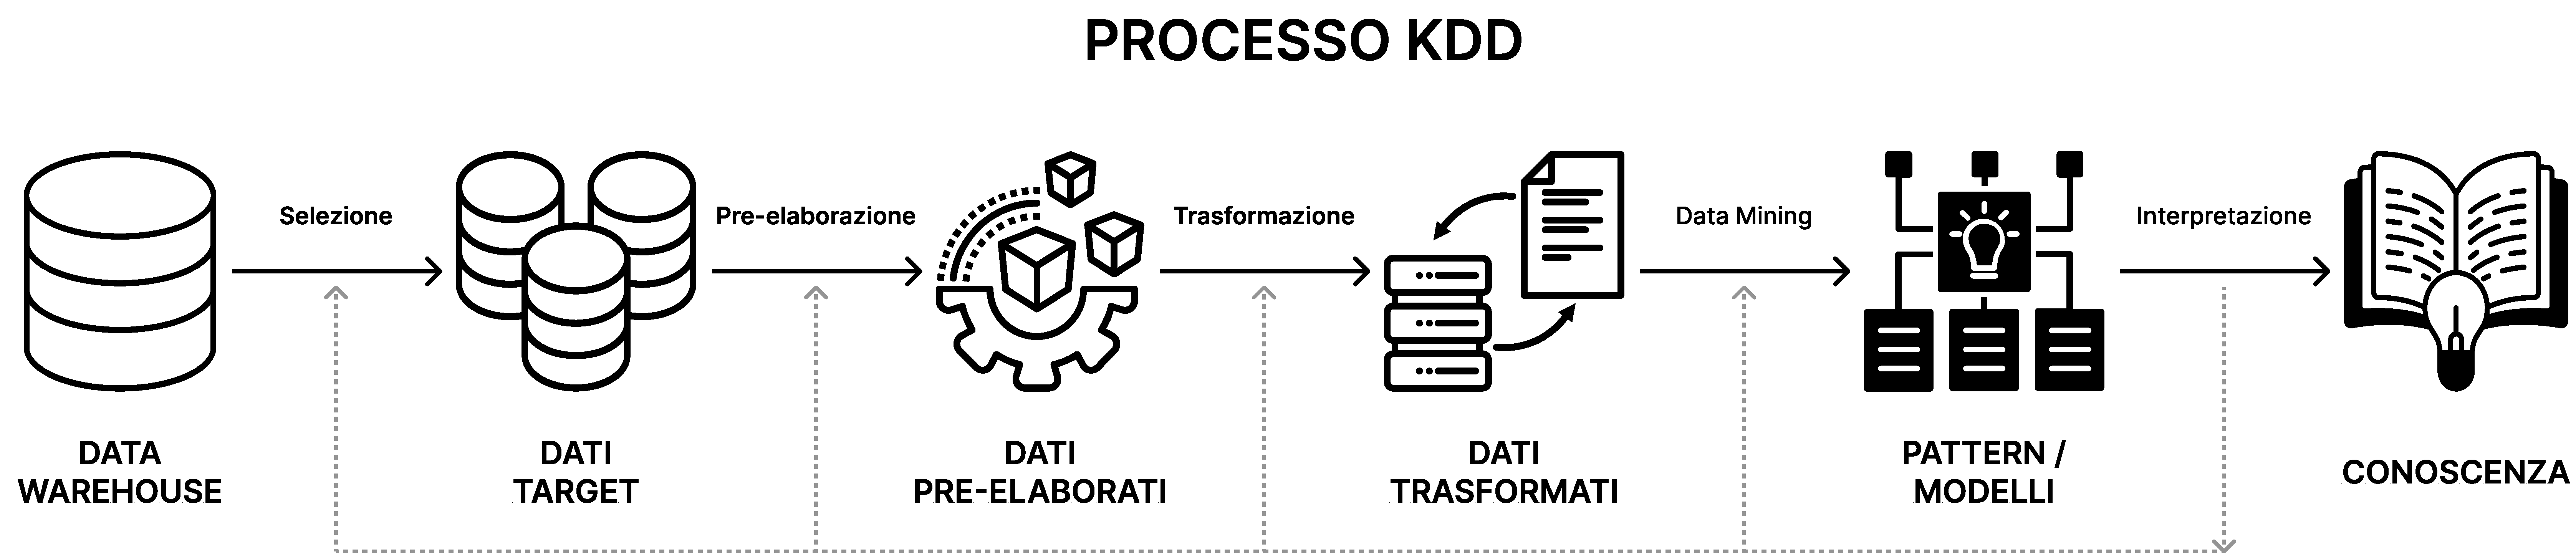
\includegraphics[width=0.75\linewidth]{figure//capitolo_3/KDD Process.png}
    \caption{Processo KDD}
    \label{fig:KDD Process}
\end{figure}
\end{comment}

\subsection{Data Mining}

Il \textbf{Data Mining} (\textit{DM}) è la fase di estrazione della conoscenza, essenziale in un processo di KDD, da una grande quantità di dati oppure un data warehouse. Per effettuare questa estrazione, il data mining combina l’intelligenza artificiale, l’analisi statistica e i DBMS nel tentativo di estrarre conoscenze dai dati archiviati. Più semplicemente, è possibile dire che il DM è il processo di applicazione di specifici metodi per estrarre dei pattern dai dati.\cite{citeseerx_data_mining}

Secondo Fayyad, il Data Mining svolge sei principali funzioni:\cite{aircconline_data_mining}

\begin{enumerate}
    \item \textit{Classificazione}: consiste nel trovare modelli che analizzano e classificano uno specifico dato in diverse classi predefinite.
    \item \textit{Regressione}: consiste nell’associare uno specifico dato ad una variabile di previsione con valori reali.
    \item \textit{Clustering}: consiste nell’identificare un insieme finito di categorie o cluster per descrivere i dati.
    \item \textit{Modellazione delle dipendenze} (apprendimento delle regole di associazione): consiste nel trovare un modello che descriva dipendenze significative tra le variabili.
    \item \textit{Rilevamento delle deviazioni} (rilevamento delle anomalie): consiste nello scoprire i cambiamenti più significativi nei dati.
    \item \textit{Riepilogo}: consiste nel trovare una descrizione compatta per un sottoinsieme di dati.
\end{enumerate}

Dato questa introduzione è possibile comprendere come il termine “Data Mining” è improprio rispetto al processo in sé che ha l’obiettivo, non di estrarre i dati, bensì sfruttare gli archivi di dati, laddove ne sia presente una grande quantità, per estrarne il significato o ricavarne una conoscenza che possa essere definita preziosa.\cite{aws_data_mining}

\subsubsection{Tecniche di data mining}

Il Data Mining viene adoperato utilizzando vari algoritmi e tecniche per trasformare grandi volumi di dati in informazioni utili. Di seguito ne sono riportati alcuni:\cite{ibm_data_mining}

\begin{itemize}
    \item \textit{Regole di associazione}. Corrisponde ad un metodo basato su regole per trovare relazioni tra variabili in un determinato dataset.
    \item \textit{Rete neurali}. Corrisponde all’utilizzo di apposite reti neurali, sfruttate principalmente per algoritmi di deep learning, allo scopo di elaborare i dati di formazione imitando l’iperconnettività del cervello umano attraverso strati di nodi.
    \item \textit{Albero decisionale}. Corrisponde all’adozione di metodi di classificazione o regressione per categorizzare o prevedere potenziali risultati basasti su un insieme di decisioni.
    \item \textit{K-nearest neighbor} (\textit{KNN}). Corrisponde all’uso dell’omonimo algoritmo non parametrico che classifica i punti di dati in base alla loro vicinanza e associazione con altri dati disponibili, presupponendo che dati simili si possano trovare vicini tra loro.
\end{itemize}

\subsubsection{Metodi di data mining}

Esistono molti metodi differenti di Data Mining adoperati per obiettivi altrettanto diversi. La tassonomia\footnote{La \textit{tassonomia} è la branca della scienza che studia i metodi di ordinamento in sistema degli elementi, delle conoscenze, dei dati, delle teorie appartenenti a un determinato ambito scientifico.\cite{treccani_tassonomia}} acquisisce una rilevante importanza per aiutare a comprendere la varietà di tali metodi, la loro interrelazione e raggruppamento. Per prima cosa è utile suddividere le tipologie di metodi di DM in due categorie principali: \textit{orientato alla verifica}, in cui il sistema verifica l’ipotesi dell’utente, e \textit{orientato alla scoperta}, in cui il sistema trova nuove regole e modelli autonomamente.\cite{data_mining_and_knowledge_discovery}

\begin{itemize}
    \item I metodi di verifica si occupano di valutare un’ipotesi proposta da una fonte esterna. Questi metodi sono meno associati al Data Mining rispetto alle loro controparti orientate alla scoperta, poiché la maggior parte dei problemi di Data Mining riguardano la scoperta di un’ipotesi piuttosto che la confutazione di una nota.
    \item I metodi di scoperta sono quelli che identificano autonomamente i modelli nei dati; da questi metodi è possibile svolgere un’ulteriore classificazione, ovvero è possibile dividerli in metodi di descrizione e previsione. I primi sono orientati all’interpretazione dei dati, concentrandosi sulla comprensione del loro mondo/contesto per trovare modelli e tendenze comprensibili per gli esseri umani; mentre i secondi hanno come obiettivo la creazione autonoma di un modello comportamentale, ottenendo in questo modo campioni nuovi e invisibili e permettendo una possibile previsione dei valori associati a tali campioni. Il ruolo dei metodi di previsione non si limita a questo, si occupano anche di creare dei pattern che permette una scoperta della conoscenza comprensibile e facile da analizzare.
\end{itemize}

\begin{comment}
\begin{figure}[!h]
    \centering
    \includegraphics[width=0.75\linewidth]{figure//capitolo_3/Data Mining Taxonomy.png}
    \caption{Tassonomia del Data Mining}
    \label{fig:Data Mining Taxonomy}
\end{figure}
\end{comment}

Dato che molto spesso si fa confusione con i termini e le definizioni di KDD e DM, di seguito è riportata una tabella riassuntiva che permette di capirne le differenze:\cite{geeksforgeeks_data_mining}

\begin{comment}
\begin{table}[!h]
    \centering
    \begin{tabular}{ccc}
        Parametro & KDD & DM\\
        Definizione & Processo di identificazione di modelli e relazioni validi, nuovi, potenzialmente utili e comprensibili nei dati. & Processo di estrazione di informazioni o modelli utili e preziosi da set di dati di grandi dimensioni.\\
        Obiettivo & Trovare conoscenza utile dai dati. & Per estrarre informazioni utili dai dati.\\
        Tecniche adoperate & Pulizia, integrazione, selezione, trasformazione dei dati, data mining, valutazione dei modelli e rappresentazione e visualizzazione della conoscenza. & Regole di associazione, classificazione, clustering, regressione, alberi decisionali, reti neurali e riduzione delle dimensioni dei dati.\\
        Output & Informazioni strutturate, come regole e modelli, che possono essere utilizzate per prendere decisioni o previsioni. & Modelli, associazioni o intuizioni che possono essere utilizzati per migliorare il processo decisionale o la comprensione.\\
    \end{tabular}
    \caption{Differenze tra il processo KDD ed il Data Mining}
    \label{tab:kdd_vs_data_mining}
\end{table}
\end{comment}

\section{Analisi dei dati}

Se il capitolo \ref{ch:Background} ci ha permesso di comprendere quanto i dati siano importanti e come siano diventati tali, con l'attuale ci sono stati spiegati largamente i concetti di \textit{Big Data}, \textit{Data Warehousing} e \textit{conoscenza} permettendoci di comprendere quali sono le operazioni, le infrastrutture e i modelli necessari alla loro gestione. Tutto ciò si raggruppa in un singolo macro ambito, ovvero quello dell'\textit{analisi dei dati}.

Più precisamente, l'\textbf{analisi dei dati} (o \textit{Data Analytics}) è il processo grazie al quale vengono ricavate le informazioni dai dati, precedentemente estratti, trasformati e centralizzati, per permettere di scoprire, analizzare e comprendere dei possibili schemi (o modelli) nascosti, relazioni, tendenze correlazioni e anomalie presenti al loro interno. L'obiettivo dell'analisi dei dati è quindi identificare informazioni utili, suggerire conclusioni e aiutare a prendere decisioni accurate.\cite{talend_data_analytics}

\subsection{Tipologie di analisi}
L’analisi dei dati viene utilizzata da quasi tutti i settori per aumentare la produttività e le entrate con una riduzione dei costi. Essa permette di dare un senso a grandi volumi di dati con una varietà di dati nella sua forma grezza priva di un modello di dati. Raccogliere e archiviare una quantità così elevata di dati acquisisce valore solamente se ben utilizzati e l'analisi è uno dei migliori modi per farlo.\cite{researchgate_big_data_analytics}
Tuttavia, data l’eterogeneità dei dati che degli ambiti di applicazione è necessario applicare tecniche di analisi differenti dipendentemente dalle proprie necessità. Proprio per questo motivo è possibile suddividere i modelli analitici in quattro differenti tipologie\cite{big_data_analytics_harnessing_data_for_new_business_models}:

\begin{enumerate}
    \item \textbf{Analisi Descrittiva}. Risponde alla domanda “Cosa sta accadendo?”. Corrisponde alla fase preliminare dell'elaborazione dei dati che crea un insieme di dati storici. In altre parole, gestisce ciò che accade in tempo reale e ciò che è accaduto in passato, così da comprendere le cause dei successi e fallimenti avvenuti in passato e conoscere gli eventuali argomenti su cui dover approfondire le proprie conoscenze date le tendenze attuali.
    \item \textbf{Analisi Diagnostica}. Risponde alla domanda “Perché è avvenuto?”. Essa esamina le informazioni passate per conoscere come, cosa e perché un evento è successo. In altre parole, il proprio scopo è quello di scoprire eventuali informazioni che permettano di identificare la causa principale di un problema e quindi i fattori che hanno causato direttamente o indirettamente un avvenimento.
    \item \textbf{Analisi Predittiva}. Risponde alla domanda “Cosa è probabile che accada?”. Questa analisi adopera i dati passati e presenti per prevenire cosa possa accadere in futuro, fornendo le probabilità associate all'evento in questione. Proprio a questo scopo vengono utilizzati sistemi di Data Mining associati a modelli specifici di intelligenza artificiale per svolgere l’analisi e creare i possibili scenari che potrebbero generarsi.
    \item \textbf{Analisi Prescrittiva}. Risponde alla domanda “Cosa si dovrebbe fare?”. Si dedica a riconoscere quale sia l’azione più corretta da intraprendere. Sfruttando i dati prevenienti dalle analisi precedentemente elencate, cerca di trovare la soluzione migliore tra le varie possibili. Essa va oltre la previsione dei risultati futuri, suggerendo anche i benefici dell’azione, secondo le previsioni generate, e mostrando al decisore le implicazioni di ciascuna scelta.
\end{enumerate}

\begin{comment}
\begin{figure}[!h]
    \centering
    \includegraphics[width=0.75\linewidth]{figure//capitolo_3/Analytics Models.jpg}
    \caption{Tipologie di analisi dei dati}
    \label{fig:Analytics Models}
\end{figure}
\end{comment}

\subsection{Aree di applicazione}
Come è possibile intuire, qualsiasi tipo di informazione o dato può essere sottoposta a tecniche di analisi dati, anche diverse, in base allo scopo prefissato. Tali tecniche possono svelare modelli e schemi che normalmente andrebbero persi nell'enorme quantità di informazioni disponibili da utilizzare. Tali ulteriori informazioni possono essere adoperate per perfezionare i processi aziendali (sia in ambito di efficienza temporale che economico).\cite{investopedia_data_analytics}

Proprio per questo motivo le aziende hanno spinto molto per applicare tale tecniche negli ambiti più disparati, al fine di migliorare le proprie prestazioni nei relativi business di interesse. Di seguito sono riportati alcuni di questi ambiti:\cite{bigdata4innovation_data_analytics}

\begin{itemize}
    \item \textit{Marketing}. Tali tecnologie ed algoritmi permettono, tramite un approccio consolidato, di svolgere al meglio campagne marketing a seguito di un targeting sempre più mirato verso i possibili clienti.
    \item \textit{Produzione}. Grazie a tecniche di analisi dati, fondate su machine learning e intelligenza artificiale, il mondo sta transitando ancora più velocemente ed efficientemente verso l'industria 4.0\footnote{L'\textit{industria 4.0}, nata dalla cosiddetta \textit{quarta rivoluzione industriale}, fa riferimento ad un modello di produzione e getione aziendale, che comporta l'adozione di strumenti connessi ad Internet, raccolta e analisi dei dati allo scopo di sfruttare processi di machine learning, aumentando la flessibilità della gestione delle fasi all'interno ci un ciclo produttivo aziendale.\cite{unifi_industry_4}} aumentando quindi l'interazione uomo-macchina e, quindi, consequenzialmente anche l'efficienza dei processi aziendali.
    \item \textit{Finanza}. Questo ambito sfrutta l'analisi dei dati per comprendere al meglio i trend passati e i possibili futuri cercando di analizzare i comportamenti delle persone rispetto a determinati stimoli e passioni in uno specifico mercato.
    \item \textit{Logistica}. Naturalmente, rientra in questo ambito anche lo studio di migliori algoritmi e tecniche per la conservazione e la gestione dei prodotti all'interno dei depositi. Ciò ridurrebbe non solo eventuali costi dovuti all'inefficienza dei processi presenti, ma anche eventuali tempistiche per il processamento degli ordini.
    \item \textit{Cyber Security}. Data la digitalizzazione delle aziende, è normale adoperare tecniche e metodologie atte a comprendere al meglio le possibili falle logiche nei propri sistemi interni in modo da predire e sventare potenziali problemi.
\end{itemize}

\subsection{I sistemi di supporto alle decisioni}

La rapida crescita di dati e quindi il relativo compito di doverli gestire e sfruttare al meglio ha portato ad avere una sempre maggiore necessità di supporto per la comprensione ed analisi degli stessi. Sono stati molti gli studi a riguardo che hanno riscontrato che le soluzioni prodotte dai decision maker sono al di sotto del loro possibile potenziale poiché essi non sono in grado di assimilare l'elevato numero di informazioni per poter svolgere il proprio compito. Per sopperire a tale problema, sono stati ideati dei \textit{sistemi di supporto alle decisioni}, o \textit{Decision Support Systems} (\textit{DSS}), ovvero strumenti che assistono direttamente i responsabili delle decisioni esecutive nel proprio lavoro semplificando le informazioni da dover sfruttare.\cite{dss_introduction}

La maggior parte delle ricerche sui DSS adotta uno dei seguenti concetti:\cite{mit_keen_dss}

\begin{itemize}
    \item Un DSS è definito in base alla struttura del compito che deve affrontare.
    \item I DSS richiedono una strategia di progettazione che sia distintiva dipendentemente dalle tecniche di evoluzione e "middle-out".
    \item I DSS supportano i processi cognitivi dei singoli responsabili delle decisioni; la ricerca decisionale fornisce approfondimenti descrittivi sulla risoluzione dei problemi di gestione e teorie normative per definire come migliorarne l'efficacia.
    \item I DSS riflettono una strategia di implementazione per rendere i computer utili ai dirigenti; questa strategia si basa sull'uso di intermediari esperti, servizi reattivi e interfacce software user-friendly.
\end{itemize}

Più precisamente, un Decision Support System è un sistema informativo che aiuta un'azienda nel compito di svolgere attività decisionali che richiedono giudizio, determinazione e una determinata sequenza di azioni. Il DSS asiste la gestione di medio e alto livello dell'azienda che lo adotta analizzando enormi volumi di dati e accumulando informazioni che possono rendersi utili per la risoluzione di problemi o la presa di decisioni.\cite{cfi_dss}

\begin{comment}
\begin{figure}
    \centering
    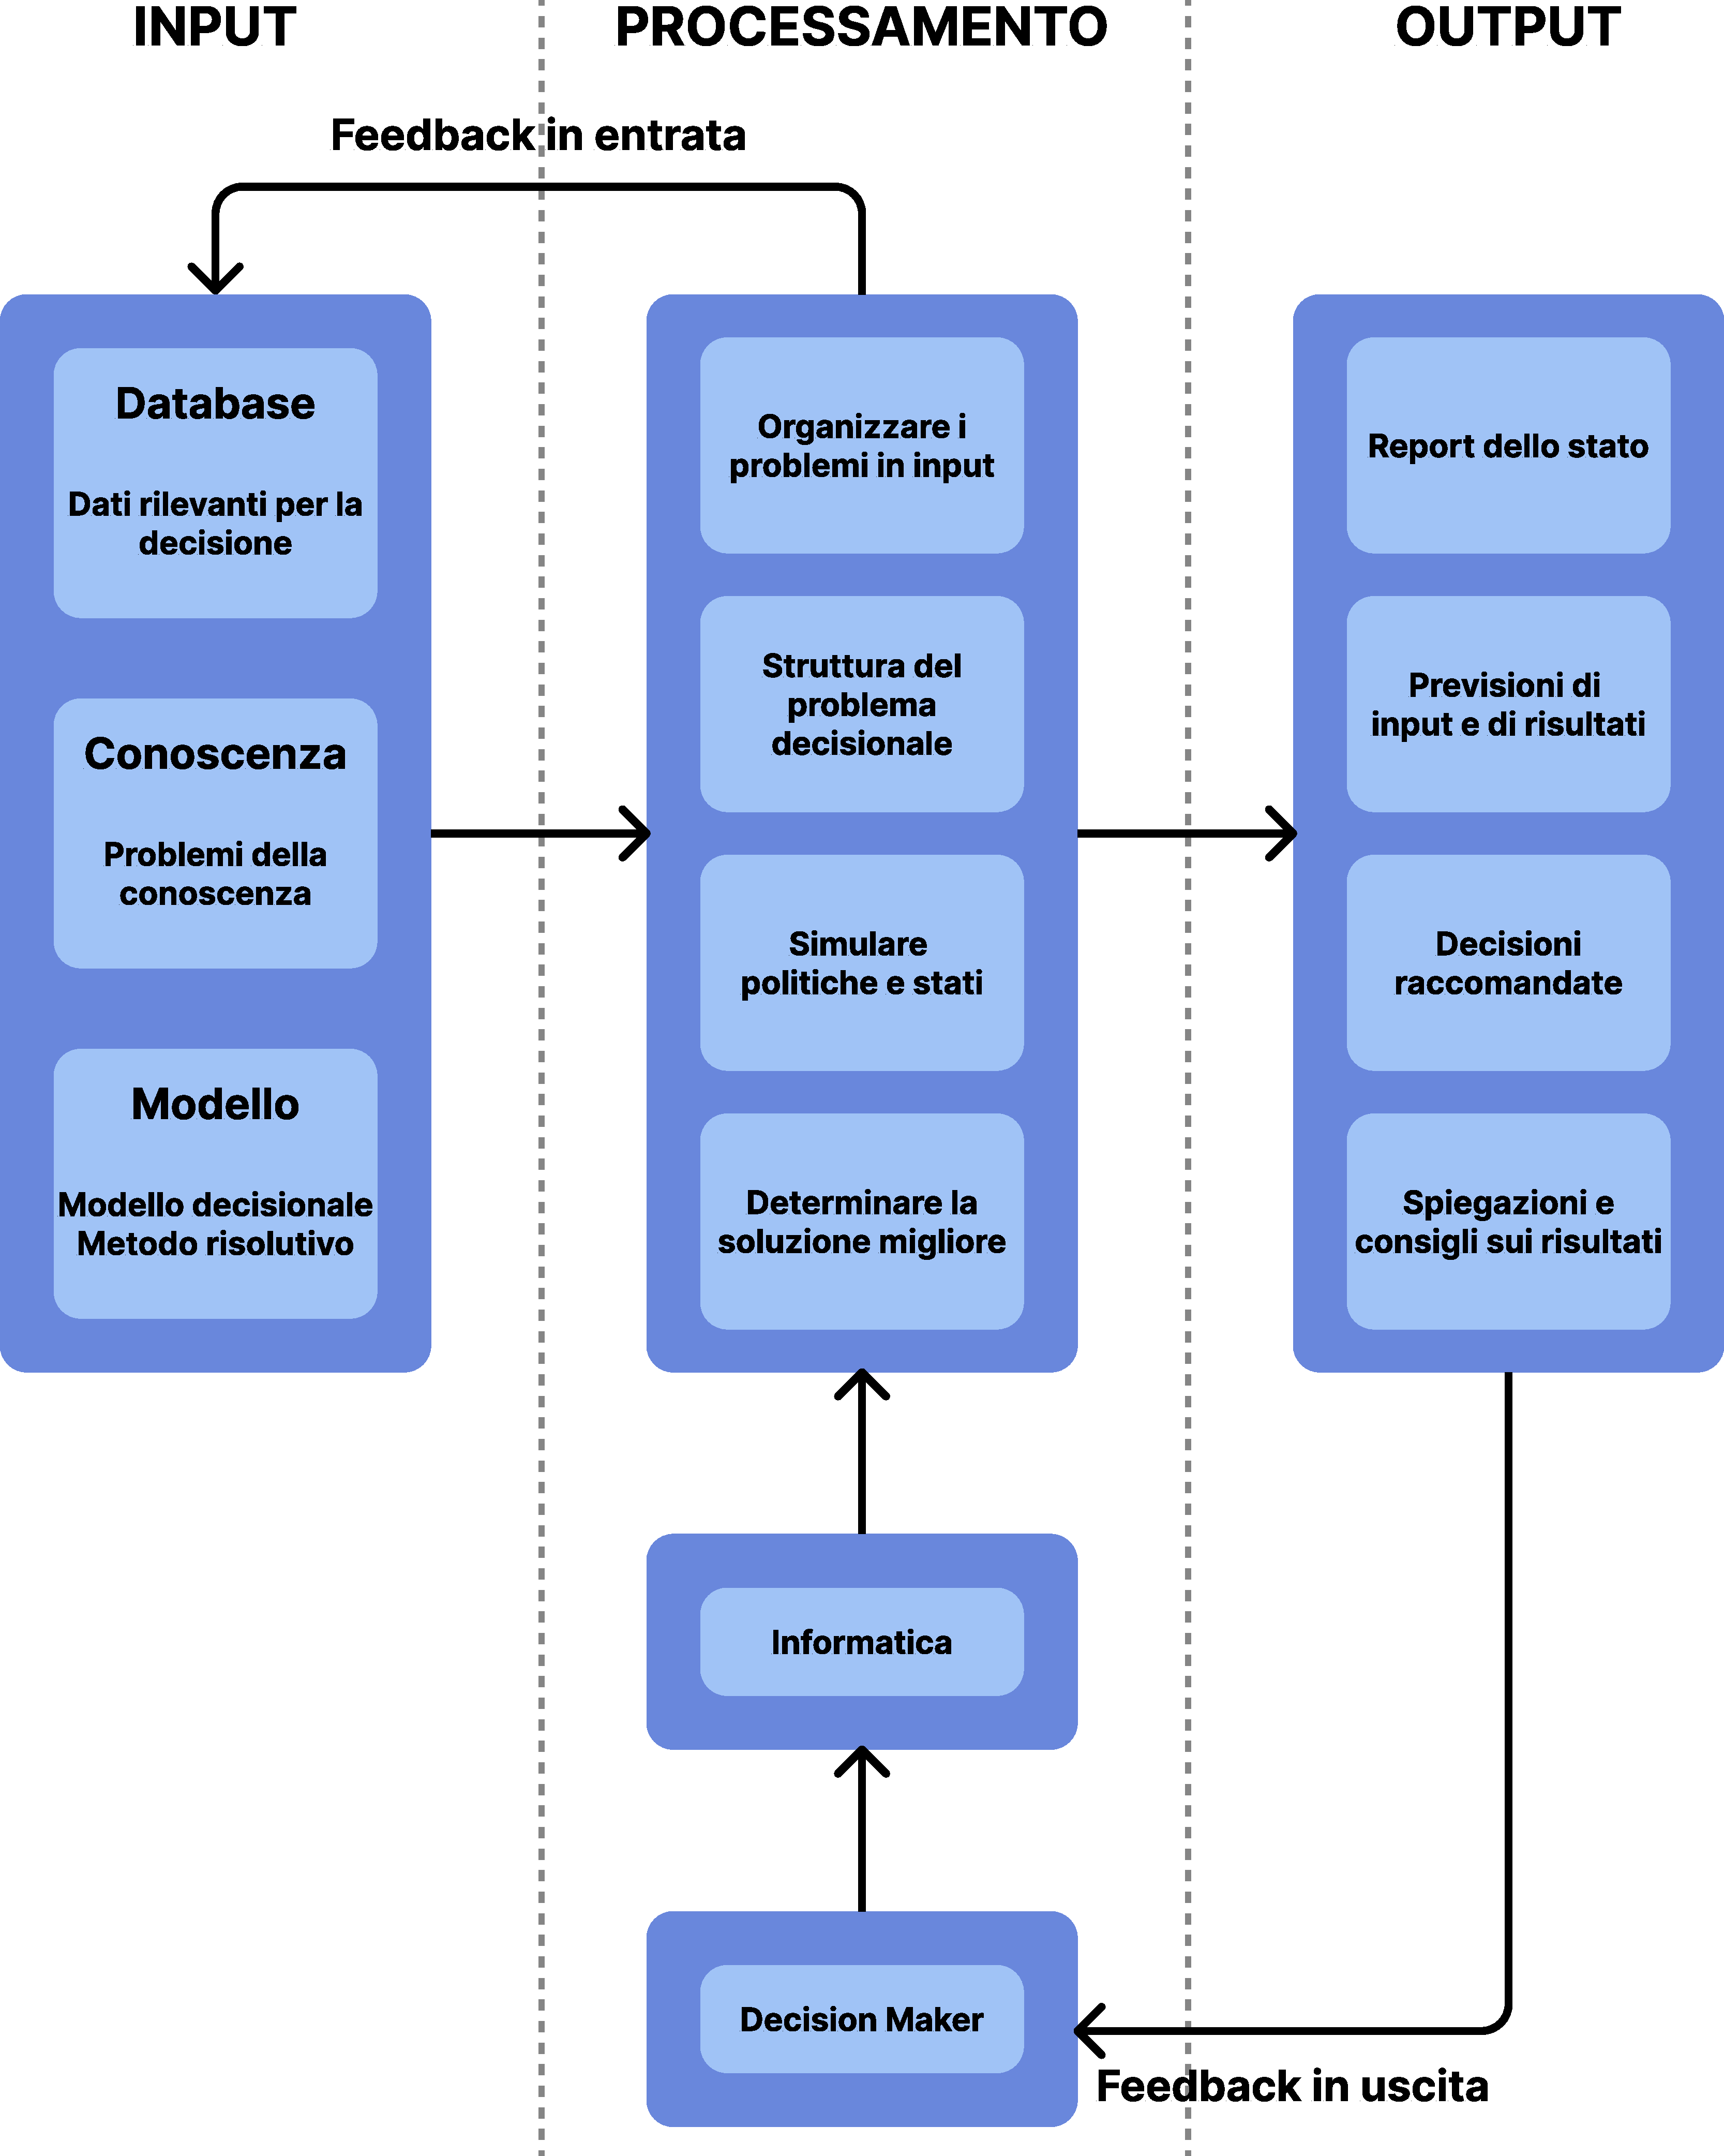
\includegraphics[width=0.75\linewidth]{figure//capitolo_4/Decision Support System Structure.png}
    \caption{Struttura di un sistema decisionale di supporto}
    \label{fig:Decision Support System Structure}
\end{figure}
\end{comment}

\subsubsection{Le caratteristiche}

Identificare le caratteristiche di un sistema decisionale di supporto non è un compito semplice data l'eterogeneità di quest'ultimi e degli ambiti in cui sono adoperati, tuttavia Turban e Aronson sono riusciti a ricapitolare quali siano le caratteristiche generali che li contraddistinguono:\cite{dss_characteristics}

\begin{itemize}
    \item Un DSS assiste i decision maker con la risoluzione di problemi semi e non strutturati facendo uso del giudizio umano e dei computer.
    \item Un DSS copre un ampio spettro di livello di gestione, dal mondo dirigenziale a quello operativo.
    \item Un DSS fornisce supporto indifferente ad individui singoli o gruppi.
    \item Un DSS facilita la presa di decisioni indipendenti e/o sequenziali che possono essere prese una o più volte.
    \item Un DSS gestisce tutte le fasi del processo decisionale, ovvero: raccolta di informazioni, progettazione, scelta ed implementazione.
    \item Un DSS copre un'ampia varietà di strumenti di analisi delle decisioni.
    \item Un DSS è adattabile e flessibile, permettendo agli utendi di aggiungere, modificare, eliminare o riorganizzare gli elementi base di cui si compone.
    \item Un DSS dovrebbe essere user-friendly.
    \item Un DSS ha l'obiettivo di migliorare l'efficacia della presa di decisioni (appropriatezza e qualità) anziché l'efficienza (il costo della presa di decisioni).
    \item Un DSS deve assistere e non sostituire un decision maker.
    \item Un DSS adotta diversi modelli di analisi per creare strategie diverse dipendentemente dalla situazione in cui si riscontra il problema.
    \item Un DSS dovrebbe essere in grado di fornire accesso a una varietà di fonti e formati differenti di dati.
    \item Un DSS può essere integrato con altri sistemi e può essere distribuito tramite tecnologie di rete e web per essere facilmente fruibile.
\end{itemize}

\subsubsection{Tipologie di DSS}

I sistemi di supporto alle decisioni possono essere suddivisi in differenti categorie dipendentemente dal principio su cui si basano, ovvero:\cite{techtarget_dss_types}

\begin{itemize}
    \item \textit{Basati sui dati}. Questa tipologia basa il proprio supporto sui dati provenienti da database (interni o esterni) sfruttando principi di data mining per poterli analizzare e mostrare all'utente.
    \item \textit{Basati sui modelli}. Questa tipologia basa il proprio supporto sull'analizzare una situazione che corrisponda ad un modello/schema precedentemente definito in base ai requisiti dell'utente.
    \item \textit{Basati sulla comunicazione e DSS di gruppo}. Questa tipologia basa il proprio supporto sull'adottare diversi strumenti di comunicazione (di ogni genere) per consentire a più di una persona di lavorare su una specifica attività, con l'obiettivo di migliorare il valore delle scelte dovute ad una collaborazione tra più persone.
    \item \textit{Basati sulla conoscenza}. Questa tipologia basa il proprio supporto sull'utilizzo di una conoscenza aggiornata continuamente e gestita da un sistema di Knowledge Mangament in modo da fornire informazioni sempre aggiornate e coerenti basate sulla conoscenza generale dell'azienda.
    \item \textit{Basati sui documenti}. Questa tipologia basa il proprio supporto sull'analisi dei documenti (interni o esterni) per rispondere a ricerche specifiche degli utenti e fornirgli le informazioni necessarie. 
\end{itemize}


\subsection{BI e BA}
Come detto in precedenza, l'analisi dei dati è un termine ampio utilizzato per comprendere diverse metodologie di analisi dei dati. Tra queste metodologie due delle più rilevanti in ambito aziendale sono sicuramente la \textit{Business Intelligence} (\textit{BI}) e la \textit{Business Analytics} (\textit{BA}) (che inoltre, possono essere identificati anche come dei DSS).

In termini generici, la BI e la BA si riferiscono all'infrastruttura collettiva, agli strumenti, alle applicazioni e ad altre risorse che generano dati e informazioni, che a loro volta valorizzano il modo in cui le aziende prendono decisioni, scoprono opportunità di guadagno e esaminano le proprie prestazioni.\cite{hpe_bi_and_a}

Di seguito sono riportate delle spiegazioni generali per comprenderle meglio.\cite{academiaedu_bi_and_ba}

\begin{itemize}
    \item \textit{Business Intelligence}. La BI può essere descritta come un insieme di tecniche e strumenti che permettono l'acquisizione e la trasformazione di dati grezzi in informazioni importanti ed utili per fini aziendali. Tali tecniche sono in grado di gestire enormi quantità di dati (strutturati e in alcuni casi anche non) per permettere l'identificazione, lo sviluppo e la creazione di nuove opportunità strategiche utili alla compagnia.
    \item \textit{Business Analytics}. La BA può essere descritta come l'insieme di competenze, tecnologie e pratiche atte all'esplorazione continua e iterativa delle prestazioni passate di una compagnia al fine di ricavare possibili intuizioni ed aiutare quindi la pianificazione delle decisioni aziendali. Tali tecniche si concentrano sullo sviluppo di nuove intuizioni e sulla comprensione delle prestazioni aziendali passate basandosi su dati e metodi statistici, in modo da migliorare le future.
\end{itemize}